\section{The ``M'' Problems}

%\renewcounter{Exercise}[subsection]
\counterwithin{Exercise}{subsection}
\renewcommand{\theExercise}{{\thesubsection}\arabic{Exercise}}
%\renewcommand{\ExerciseHeaderNB}{M\Alph{\subsection}\arabic{\Exercise}}
%\renewcommand{\ExerciseHeader}{\textbf{M\Alph{subsection}\ExerciseHeaderNB.\ExerciseHeaderDifficulty}}
\renewcommand{\ExerciseHeaderNB}{\thesubsection\arabic{Exercise}}
\renewcommand{\ExerciseHeader}{\textbf{\ExerciseHeaderNB.\ExerciseHeaderDifficulty}}
\renewcommand{\AnswerHeader}{\textbf{\ExerciseHeaderNB.} }
%\setlength{\AnswerSkipBefore}{0pt}
%\setlength{\AnswerSkipAfter}{0pt}
\setlength\Exerightmargin{3in}
\renewcommand{\AtBeginAnswer}{\setlength\Exerightmargin{3in}\hangindent=0.7cm}

%\numberwithin{Exercise}{subsection}

\titleformat{\subsection}{\normalfont\large\bfseries}{\thesubsection~Problems:}{1ex}{}

%\renewcommand{\sectionmark}[1]{\markboth{\MakeUppercase{\thesection:\ #1}}{}}
\renewcommand{\subsectionmark}[1]{
   \markright{\thesubsection~Problems: #1}}

\subsection{Waves and Velocity} 

(Answers to M\Alph{subsection} problems are on page \pageref{waves_and_velocity_prob_answers}.)

\begin{Exercise}
If you haven't done so already, please read the following documents on Blackboard under ``Course Information:''
\begin{itemize}[nosep]
\item The Syllabus
\item ``On Working Together Honestly''
\item Homework Guidelines
\end{itemize}
(a)~If you could change any aspect of these course policies (or anything else about the course, I guess), what would you change?  You must make at least one suggestion for a change; no fair just answering that you're fine with whatever's currently there.  (b)~How serious are you about this request?  (Are you just suggesting a change because it was required, or because you genuinely think it would improve the course?)
\end{Exercise}

\begin{Exercise}[difficulty=1]
Use Appendix A in the lab manual to help you answer these dad jokes.  (a)~What do you call one millionth of a phone?  (b)~What do you call $2 \times 10^3$ mockingbirds? (c)~What do you call $1 \times 10^{-12}$ of a ``boo''?  (d)~What do you call one billionth of one billionth of a miser?  (e)~What do you call $10^{-6}$ meter? (this one's not actually a dad joke, but a serious question.) (f)~What space vessel held the dubious distinction of completing the Kessel Run in ``under 12 parsecs''?
\end{Exercise}

\begin{minipage}{0.74 \textwidth}
\begin{Exercise}[difficulty=1]
The right triangle shown in the figure has sides of length $A$, $B$, and $C$, and one of the angles is $\theta$.  (a)~Write an expression for $A$ in terms of $C$ and $\theta$.  (b)~Write an expression for $B$ in terms of $C$ and $\theta$.  
\answerspace{0.2in}
\end{Exercise}
\end{minipage}
\begin{minipage}{0.25 \textwidth}
\hspace{\fill}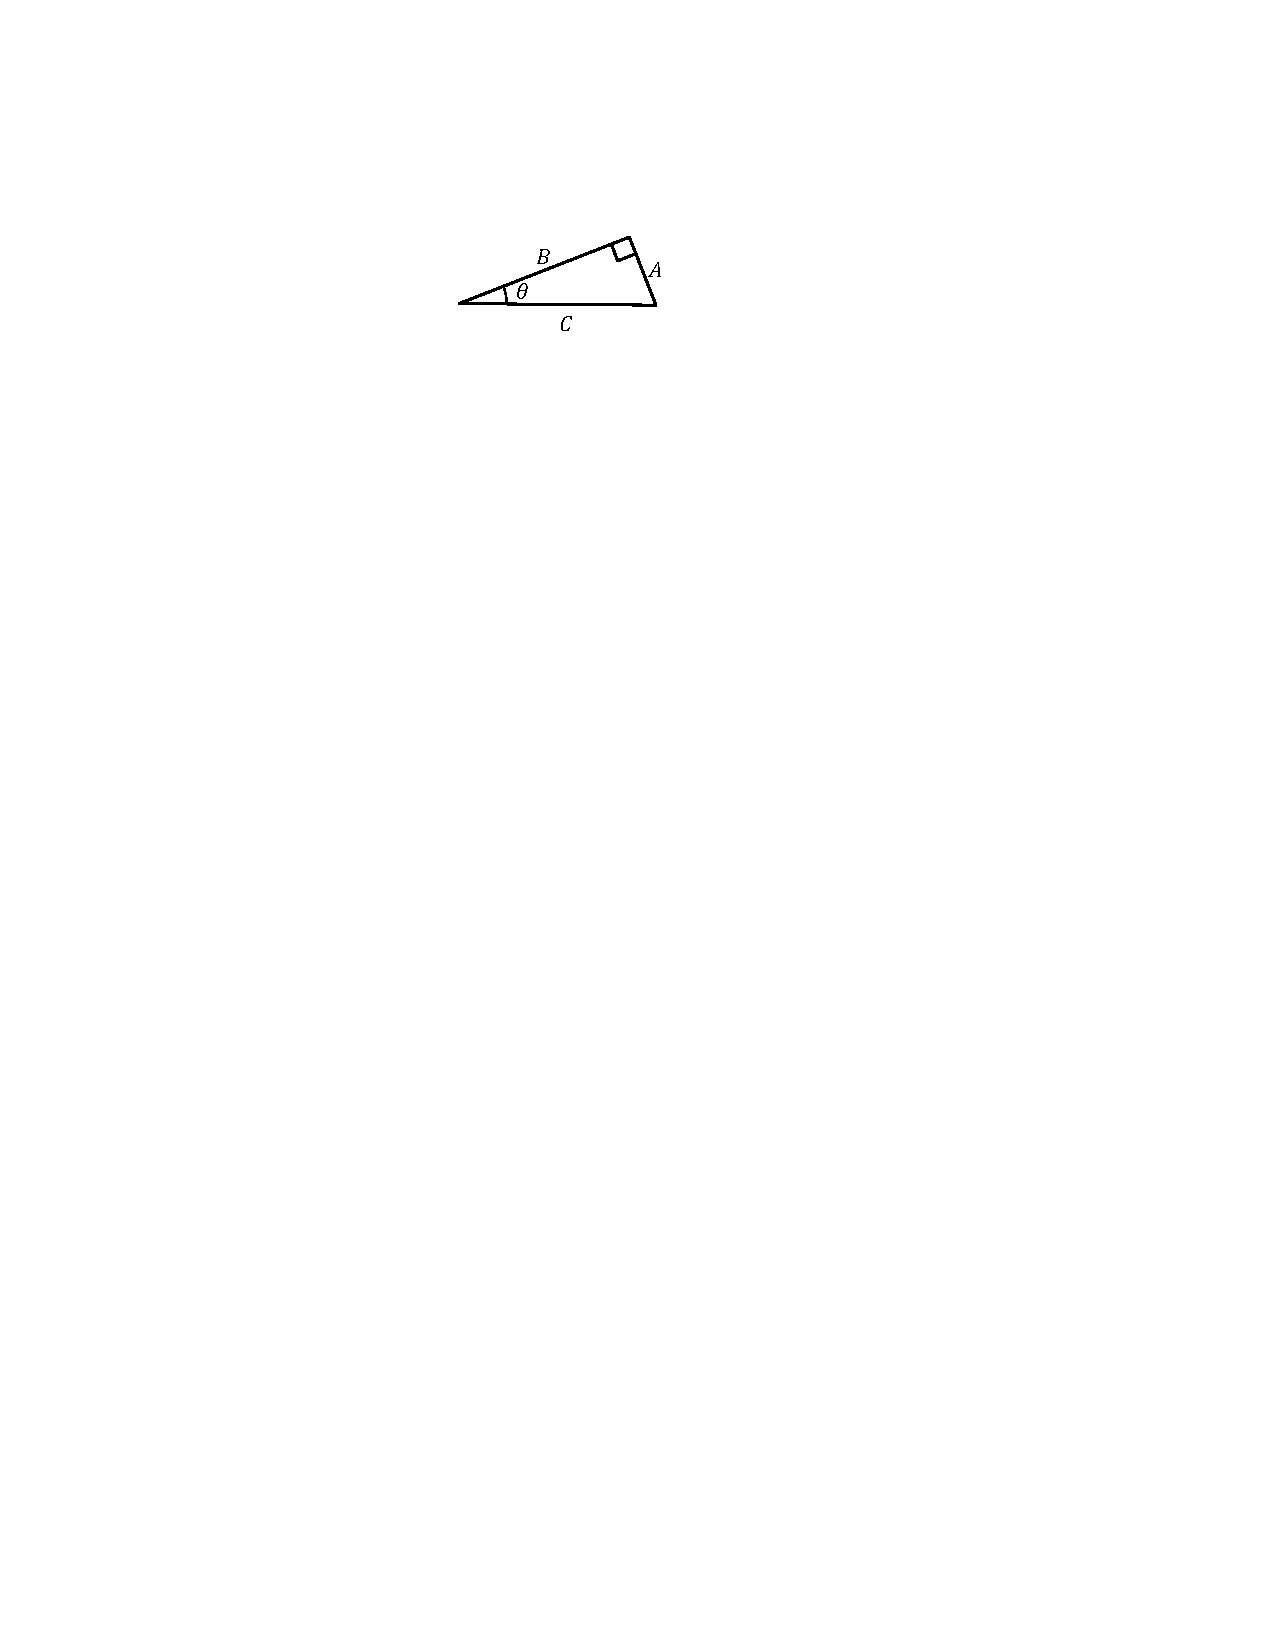
\includegraphics{M_problems/waves_velocity/triangle.pdf}
\end{minipage}
\begin{Answer}
(b) $B=C \cos\theta$
\end{Answer}

\begin{Exercise}[difficulty=1]
How long does it take for light to travel the distance of $L=80$~cm between the pair of slits and the detector in the experiment we did?  (The speed of light $c$ is $3 \times 10^8$~m/s, a value you will need to know for the rest of this course.)
\end{Exercise}
\begin{Answer}
2.67 ns
\end{Answer}

\begin{Exercise}
The nearest star to us is Proxima Centauri, which is 4.2465 light-years away from us.  If we could send a probe to that star at a constant speed one tenth of the speed of light ($v=0.1c$), how long would it take the probe to go there, snap one picture, and then return to Earth?
\end{Exercise}
\begin{Answer}
84.93 years
\end{Answer}

\begin{Exercise}
Imagine you are doing an experiment as in Lab~\ref{interference_lab}, shining light through two slits and observing the series of bright and dark spots created on a distant screen.
\begin{enumerate}[nosep,label=(\alph*)]
\item Suppose you increase the wavelength $\lambda$ of the light that you are using.  Does that make the bright spots on the screen \textit{closer together}, \textit{further apart}, or \textit{no change}?  
\item Now suppose that you keep the wavelength $\lambda$ of the light the same, but instead you increase the spacing $d$ between the two slits.  Does that make the bright spots on the screen \textit{closer together}, \textit{further apart}, or \textit{no change}?  
\item Finally, suppose you keep both $\lambda$ and $d$ the same, but instead you increase the distance $L$ from the slits to the screen.  (Say you increase it from 80~cm to 100~cm, for instance.)  Does that make the bright spots on the screen \textit{closer together}, \textit{further apart}, or \textit{no change}?  
\end{enumerate}
For parts (a) and (b) of this problem, it's worth thinking about each part for a few minutes with a pencil and paper, but then you should definitely check your answers using the little Mathematica applet interference.cdf that you used in class, which is available on Blackboard under ``Labs''.
\end{Exercise}
\begin{Answer}
(c) Increasing $L$ will increase the distance between bright spots on the screen.
\end{Answer}

\begin{Exercise}
Green laser light with a wavelength of $\lambda = 500$~nm is incident on two slits, separated by a distance $d=125~\mu$m, projecting a series of light and dark spots onto a distant screen, just as you did in Lab~\ref{interference_lab}.  Suppose that at one specific place on the screen, slightly to the left of the center, the distance from that spot on the screen to one of the two slits is exactly $1.75~\mu$m greater than the distance to the other slit.  (That is, the path difference $\Delta r$, in the diagram in Activity 3 of your lab, is exactly $\Delta r=1.75~\mu$m.)  Is that specific place on the screen a bright spot, or a dark spot?
\end{Exercise}
\begin{Answer}
It's a dark spot.  Of course, on your homework paper, you need to show your work and explain \textit{why} it's a dark spot.  Oh, by the way: yes, this problem does include an extraneous piece of information that you didn't need---you're welcome!  :-)
\end{Answer}


\begin{Exercise}
Laser light is incident on a pair of slits separated by a distance of $90~\mu$m.  When a screen is placed 1.4~meters behind the slits, bright spots on the screen are observed to be separated from each other by a distance of 8.3~mm.  What is the apparent wavelength of the laser light?
\end{Exercise}
\begin{Answer}
534~nm
\end{Answer}

\begin{Exercise}
Laser light with wavelength $\lambda=655$~nm is incident on a set of three narrow slits.  The outer slits are exactly $150~\mu$m apart, and a third slit lies exactly midway between them.  (a)~Consider only a set of rays directed at an angle
$\theta=0.25^\circ$ from horizontal.  When these rays eventually reach a screen (or a detector), will they combine in such a way that they produce an interference maximum, an interference minimum, or something in between?  (b)~If a screen is placed 1.25~meters away from these slits, at what locations $\Delta x$ relative to the centerline will the first three intensity maxima be found?
\begin{center}
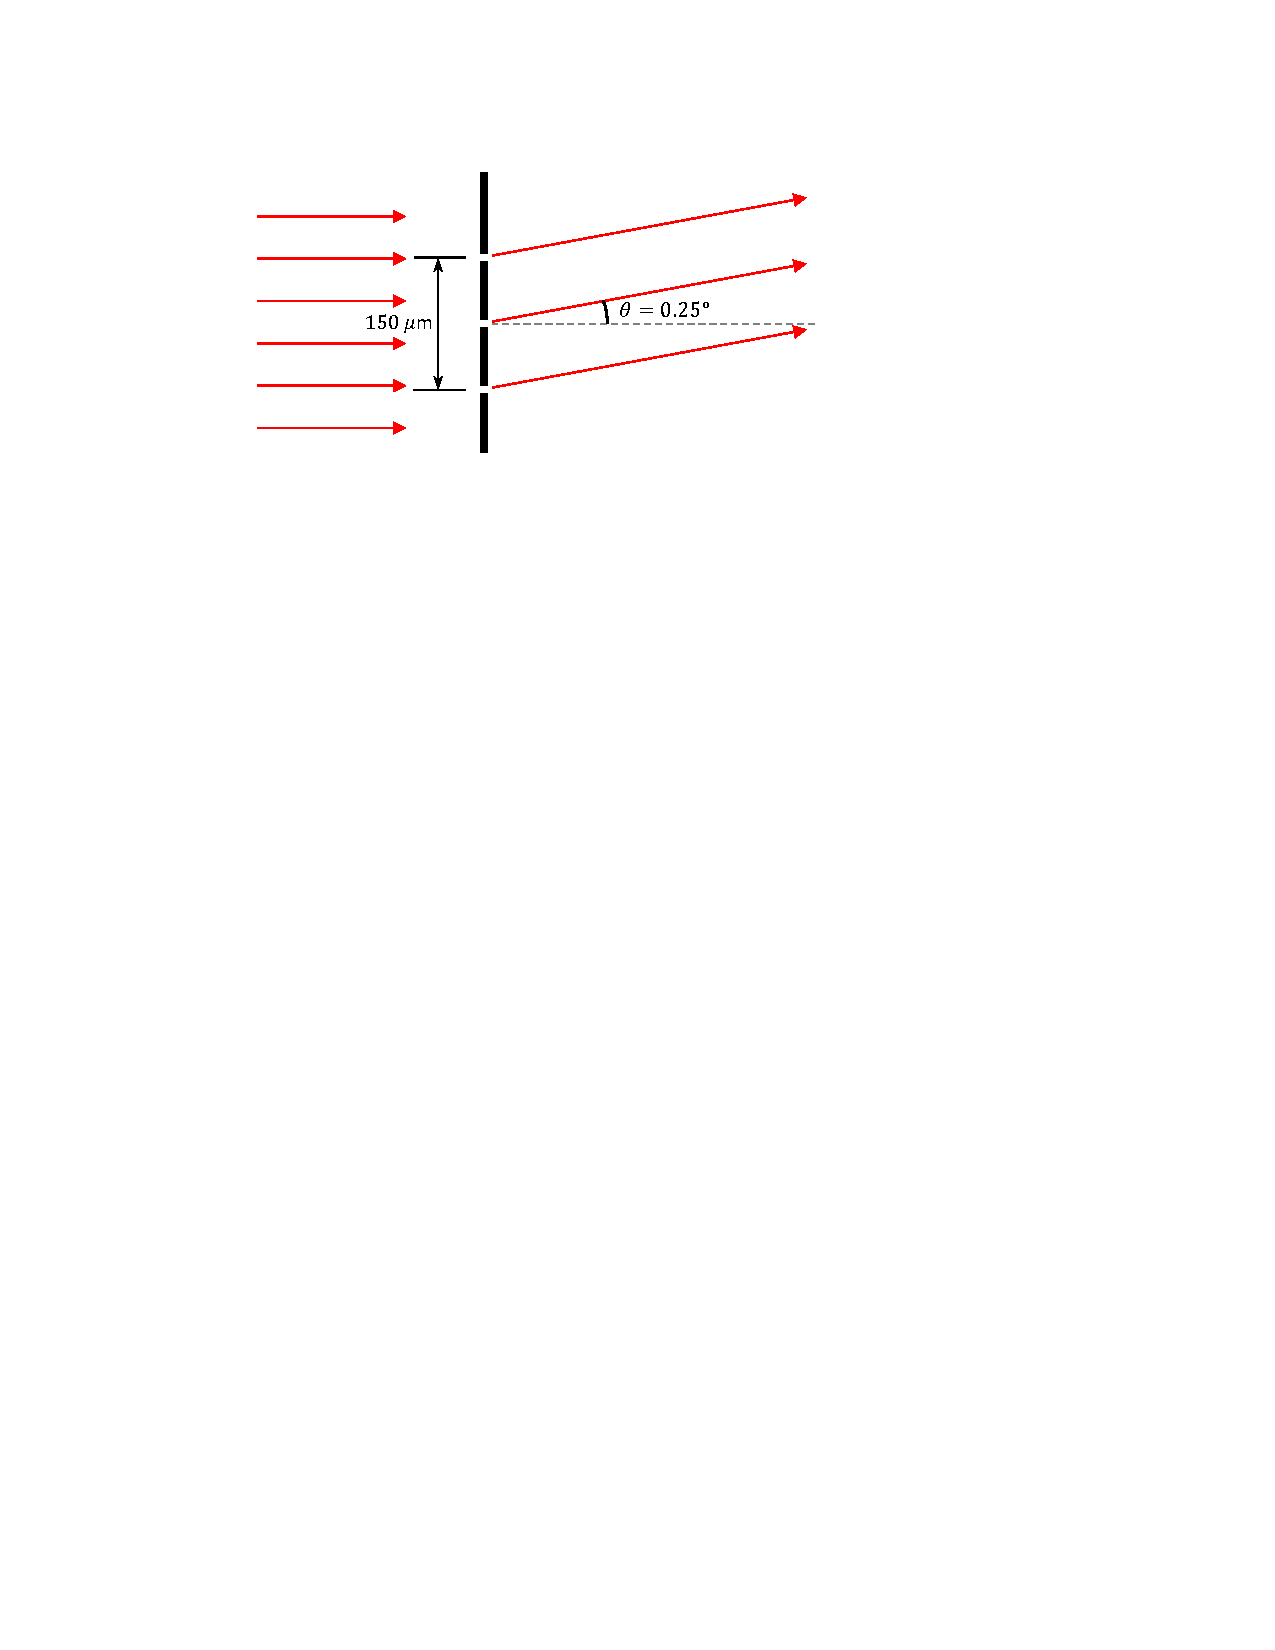
\includegraphics[scale=0.9]{M_problems/waves_velocity/three_slits.pdf}
\index{color page}
\end{center}
\end{Exercise}
\begin{Answer}
(a) Something in between.  (b) $\Delta x=0$~mm, $\pm 10.9$ mm, and $\pm 21.8$ mm.
\end{Answer}


\begin{Exercise}
Use the little Mathematica applet \filename{interference.cdf} that we've used in class to answer this question.  Start with two slits, and then increase the number of slits from 2 up to 3, 4, and 5.  (a)~As you increase the number of slits, what happens to the locations of the bright spots on the distant screen?  (b)~As you increase the number of slits, what happens to the intensity, or maximum brightness, of each bright spot?  (c)~As you increase the number of slits, what happens to the width of each bright spot?  (d)~Is a location on the screen that is an exact brightness minimum for two slits also always an exact brightness minimum for 3, 4, or 5 slits? \label{problem_number_of_slits}
\end{Exercise}

\begin{Exercise}
A ``diffraction grating'' is what you call a device with hundreds or thousands of slits for light to pass through, as opposed to just two or three or a dozen slits.  As you saw in problem \ref{problem_number_of_slits}, when you add more slits, the locations of the brightness maxima and minima do not change; you still have constructive interference at any angles for which 
$d \sin \theta = m\lambda$,
where $m$ is any integer.  
Suppose you shine red laser light with a wavelength of 625~nm on a diffraction grating with many slits, all spaced $3.5~\mu$m apart.
Calculate all of the angles $\theta$ at which constructive interference (bright spots) will be observed.
\end{Exercise}
\begin{Answer}
$0^\circ$, $10.3^\circ$, $20.9^\circ$, $32.4^\circ$, $45.6^\circ$, and $63.2^\circ$
\end{Answer}

\begin{Exercise}[difficulty=1]
Draw a quantitative position vs. time graph for the following motion, as you walk back and forth along an $x$ axis: 
\begin{itemize}[nosep]
\item You start at a position $x=+2$ m at time $t=0$.
\item First, you walk in the negative $x$ direction at a velocity $v=-2$ m/sec for 3 seconds.
\item Then you stop for 3 seconds.
\item Finally, you walk in the positive $x$ direction at velocity $v=+1$ m/sec for 3 seconds.
\end{itemize}
Note that ``quantitative'' means that your axes should have numbers, so a person looking at your graph could read a specific numerical value of your position at any given time from your graph.
\end{Exercise}


\begin{Exercise}
A cat is chasing a mouse across a large, 10-meter-wide room.  The cat starts at one end of the room, $x=0$, and runs at top speed ($v=6$~m/s) towards the mouse, who is at the center of the room, $x=5$~m.  At the same time, the mouse runs at $v=4$~m/s away from the cat, towards a mouse hole at the far end of the room, $x=10$~m.  (a)~Draw a single position vs. time graph with two lines on it, one representing $x$ vs. $t$ for the cat, and one representing $x$ vs. $t$ for the mouse.  (b)~Perhaps you remember from previous math classes that the general equation for a line is $y=mx+b$, or, in this case, $x=vt+x_0$, where $x_0$ represents the position at time $t=0$. Write an equation describing the position of the cat as a function of time, $x_{\rm cat}(t)$, using the numbers in this problem.  (c)~Write another equation for the position of the mouse as a function of time, $x_{\rm mouse}(t)$.  (d)~Does the mouse get away?
\end{Exercise}
\begin{Answer}
(b) $x_{\rm cat} =(6~{\rm m/s})t+0$ m  (d)~Hint: if the mouse does NOT get away, that would mean that there's some time $t$ when $x_{\rm cat} =x_{\rm mouse}$  that occurs BEFORE the mouse gets to the hole, right? 
\end{Answer}

\begin{Exercise}
From the pages from Griffiths' book Electrodynamics that are posted under ``Notes,'' give three examples of equations that are integrated into sentences or introduced differently from anything you did in your first writing assignment. For each example, write the sentence and say something intelligent about how the equation (or a part of the equation) functions in the sentence.  (For instance, does the equation function as the main clause of the sentence?  Or as a subordinate clause?  Is one of the variables in the equation obviously identifiable as the subject or predicate nominative of the sentence? If you are unsure of these grammatical terms, you can focus instead on the ways in which variables are defined either before or after the sentence, for instance by using ``where,'' after the equation, or in an appositive before the equation, etc.) 
\end{Exercise}



\bigskip\bigskip\bigskip
\pagebreak[3]
\textbf{Answers to Selected {\thesubsection} Problems:}
\label{waves_and_velocity_prob_answers}
%\shipoutExercise
\shipoutAnswer

\cleardoublepage

\subsection{Galilean Relativity} 

(Answers to M\Alph{subsection} problems are on page \pageref{galilean_relativity_prob_answers}.)


\begin{Exercise}[difficulty=1]
(a) Draw a Minkowski diagram depicting the following motion, as you walk back and forth along an $x$ axis: 
\begin{itemize}[nosep]
\item You start at a position $x=+2$ m at time $t=0$.
\item You walk in the negative $x$ direction at a velocity $v=-2$ m/s for 3 seconds.
\item Then you stop for 3 seconds.
\item Finally, you walk in the positive $x$ direction at velocity $v=+1$ m/sec for 3 seconds.
\end{itemize}
(b)~Write the $(x,t)$ coordinates of four specific ``events'' at which your motion changes.  
(c)~Use the Galilean transformations to transform the coordinates of those four events into new coordinates $(x',t')$ in different reference frame $S'$ which moves with velocity $v=-1$~m/s relative to the original frame $S$.  
(d)~Draw a Minkowski diagram depicting your motion in the $S'$ reference frame.  
(e)~What is your maximum velocity $u'$ in the $S'$ frame, and when does it occur?  
(f)~Use the Mathematica notebook file minkowski\_events.nb to check your answers.  What are the maximum and minimum values of frame velocity $v$ that are available to you in this simulation?
\end{Exercise}
\begin{Answer}
(c) (2 m, 0 s), (-1 m, 3 s), (2 m, 6 s), and (8 m, 9 s)  (e) max $u'=+2$ m/s.  When is that? 
\end{Answer}


\begin{Exercise}[difficulty=1]
A reference frame $S'$ moves in the $-x$ direction relative to frame $S$ with velocity $v=-20$~m/s.  An object moves back and forth along the $x$ axis, viewed by observers in both frames.  (a)~What is the object's velocity $u'$ in frame $S'$ if its velocity in frame $S$ is $u=+100$~m/s?  (b)~What is the object's velocity $u'$ in frame $S'$ if its velocity in frame $S$ is $u=-100$~m/s?  (c)~Suppose the object has a velocity in frame $S'$ of $u'=50$~m/s.  What is its velocity in frame $S$?
\end{Exercise}
\begin{Answer}
(a) 120 m/s (b) $-80$ m/s (c) 30 m/s
\end{Answer}


\begin{Exercise}[difficulty=1]
A reference frame $S'$ moves in the $+x$ direction relative to frame $S$ with velocity $v=5$~m/s.  As usual, the origins of the two frames coincide at time $t=0$.  (a)~How far apart are the origins of the two frames at time $t=10$~s?  (b)~At time $t=10$~s, an object is located at coordinates $x=80$~m and $y=20$~m in frame $S$.  At that time, what are its $x'$ and $y'$ coordinates in frame $S'$?
\end{Exercise}
\begin{Answer}
(a) 50 m apart (b) $x'=30$ m, $y'=20$ m
\end{Answer}



\begin{Exercise}[difficulty=1]
In the expression for $x$ below, $a$ and $b$ are both positive real numbers, and $a>b$:  
$$
x=\frac{2a}{(a+b)(a-b)} -\frac{a}{(a^2-b^2 )}-\frac{1}{\sqrt{a^2-b^2}} .
$$(a) Simplify the expression. 
(b) Is $x$ positive, negative, or zero, or is there not enough information to tell?  Yes, you must justify/explain your reasoning, but you don't need a full, mathematically rigorous proof.
\end{Exercise}
\begin{Answer}
(b) In fact, $x>0$. Hints: (1)~Use the ``FOIL'' (first-inner-outer-last) method to multiply $(a+b)(a-b)$. (2)~Rewrite all three terms using a common denominator; in particular, it will be helpful to ``rationalize the denominator'' in the last term.
\end{Answer}

\begin{Exercise}
Mary can paddle her kayak at a speed of 3 m/s in still water.  (a)~How long does it take her to cross a 100-m pond in her kayak?  (b)~Now suppose she paddles her kayak upstream in a river, paddling against the current, which flows at 2~m/s.  How long does it take her to paddle 100~m up the river?  (c)~How long does it take her to paddle 100~m down the river, in the same direction as the current?
\end{Exercise}
\begin{Answer}
(a) 33 seconds (b) 100 seconds (c) 20 seconds
\end{Answer}

\begin{Exercise}
Mary now turns her kayak directly across the river, which is 100~m wide.  Again, Mary can paddle at 3 m/s in still water, and the current in the river flows at 2~m/s.  
(a)~If Mary aims her canoe directly perpendicular to the current, she ends up being carried downstream by the river.  How far down the river is she carried by the time she gets to the opposite side?  
(b)~Instead, Mary aims her canoe at an angle, across the river but also upstream, so that she reaches the other side of the river at a spot directly across from where she started.  What is Mary's velocity relative to the shore?  
(c)~In part~(b), how long does it take Mary to reach the other side?
\end{Exercise}
\begin{Answer}
(a) 67 meters (b) 2.24 m/s (c) 44 seconds
\end{Answer}

\begin{Exercise}
There are three equally fast swimmers A, B, and C.  Rank the following from shortest to longest time, justifying your answer:
\begin{enumerate}[nosep,label=(\Alph*)]
\item Swimmer A swims 100 m out and 100 m back in a still lake.
\item Swimmer B swims 100 m directly across a flowing river and back to the same spot.
\item Swimmer C swims 100 m up the river (directly against the current), then back down the river, to the same spot.
\end{enumerate}
\end{Exercise}

\begin{Exercise}
Anna and Bob are having a swimming race, at a river of width $L$ flowing at speed $v_r$.  In still water, both swimmers have speed $v_s$ relative to the water.  Anna swims across the river and back, swimming at an angle against the current so that she ends up at the same place she started, without being carried down river.  Bob swims close to the shore, first upstream by a distance $L$ (relative to the bank), then downstream by distance $L$.  Calculate the time for each swimmer to cover the distance $2L$, and demonstrate which swimmer wins.  
\end{Exercise}
\begin{Answer}
$\Delta t_{\rm Anna} = 2L/\sqrt{v_{\rm s}^2-v_{\rm r}^2}=2L\sqrt{v_{\rm s}^2-v_{\rm r}^2}/(v_{\rm s}^2-v_{\rm r}^2); \Delta t_{\rm Bob} =2Lv_{\rm s}/(v_{\rm s}^2-v_{\rm r}^2 )$; Anna wins because her time is shorter.
\end{Answer}

\begin{minipage}{0.65 \textwidth}
\begin{Exercise}[difficulty=1]
The figure to the right shows a Minkowski diagram with 16 events in a reference frame $S$.  For reference, the dotted line shows the worldline of a photon that is emitted at the origin at time $t=0$ and travels in the $+x$ direction at speed $c$.  Use the Galilean transformations to show how the 16 events would appear in a space-time diagram drawn in a new reference frame $S'$, moving at speed $v=+0.5c$ with respect to the old frame $S$.  (Note: it turns out that the Galilean transformations are incorrect at high speeds, but for this exercise, please draw how the events would transform under the Galilean transformations anyway.)
\end{Exercise}
\end{minipage}
\begin{minipage}{0.34 \textwidth}
\hspace{\fill}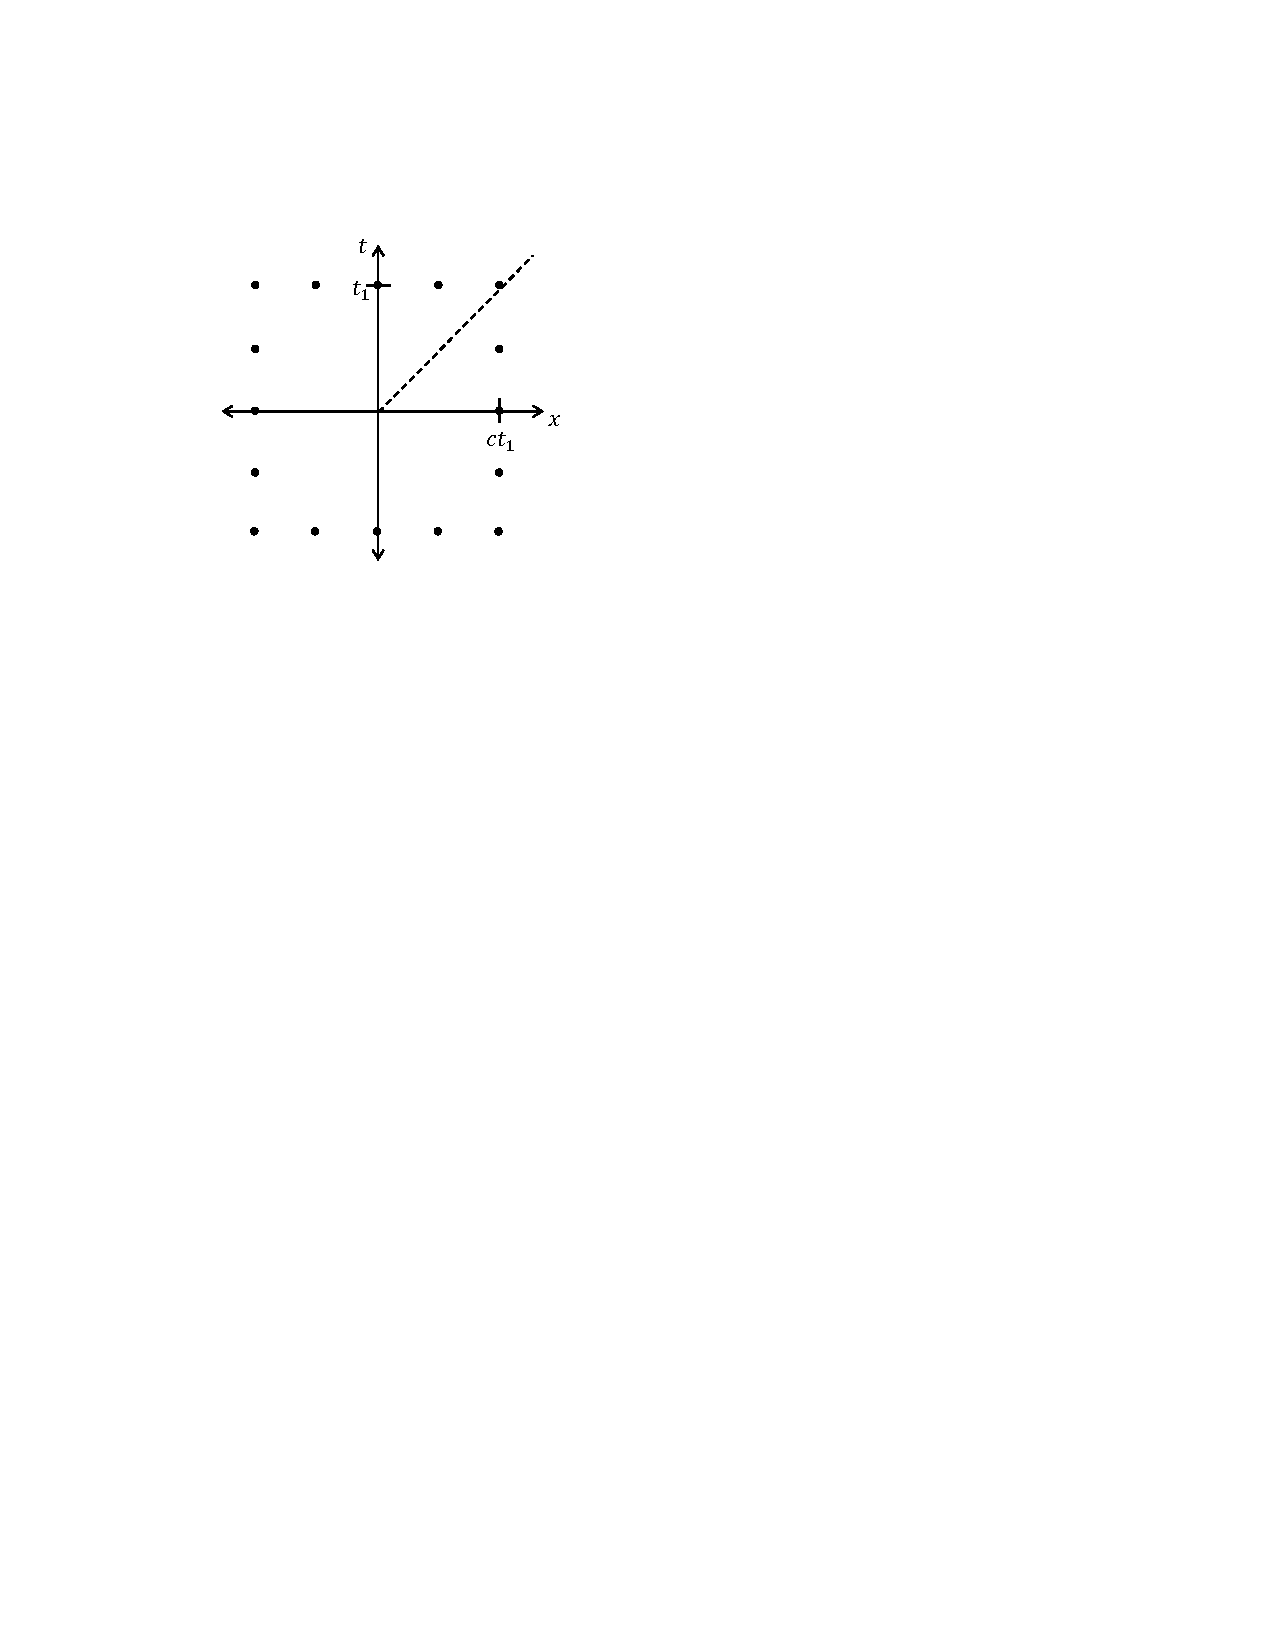
\includegraphics[scale=0.8]{M_problems/galilean_relativity/16_points.pdf}
\end{minipage}


\begin{Exercise}
\label{federation_and_romulans_prob}
A Federation spacecraft has had engine trouble and is drifting helplessly in space.  A Romulan spacecraft whizzes by at a constant velocity of $v=+0.2c$.  The Federation spacecraft radios the Romulan spacecraft and asks for help.  The Romulans answer back, ``We can't help you.  We are having engine trouble, and we are drifting helplessly in space.  We just saw you whiz by at $v=-0.2c$.  We were just about to radio you and ask for help.''  Are the reference frames of the two spacecraft equally valid?  Is there any way to tell only from the velocities of the two ships whether the Romulans are telling the truth?  Explain.
\end{Exercise}


\begin{Exercise}
The lettered parts of this problem are all related, in that they get at how the velocities of some different kinds of waves are seen in different reference frames.  \textbf{Draw a stick-figure cartoon for each situation below, along with labeled arrows showing the velocities given.} And, of course, answer the questions.
\begin{enumerate}[nosep,label=(\alph*)]
\item A luxurious limousine \href{https://veryfamousmagazine.com/glamorous-history-hot-tub-limo/}{includes an actual hot tub.}  
While the limousine is parked, you notice that when you splash your hand in the water, waves on the surface of the water travel from the back to the front at 2~m/s.  Suppose you splash your hand in the same way while the limousine is driving forward at 10~m/s.  In the reference frame of a person standing on the sidewalk as you pass by, what is the velocity of these water waves?
\item Now consider a different, regular-old-smelly-old limousine which does not include a hot tub, but is still rather long.  Inside the enclosed passenger area, sound travels at 343~m/s in air, just as it does outside.  Suppose you yell from the back of the limousine towards the driver in the front while the limousine is driving forward at 10~m/s.  In the reference frame of a person standing on the sidewalk as you pass by, what is the velocity of these sound waves?
\item Forget the limousine.  You are standing on a sidewalk, and you see your friend down the street from you, and you yell to her.  The wind is blowing from you towards your friend at 10~m/s.  In the reference frame of your friend, what is the velocity of the sound waves traveling towards her?
\item While you are still yelling to her, your friend starts to run towards you at a speedy 5~m/s.  Now, in the reference frame of your friend, what is the velocity of the sound waves traveling towards her?
\item Finally, suppose that you run towards your friend as well, at 3~m/s.  (And, to review, your friend is also running towards you at 5~m/s, and the wind is blowing towards your friend at 10~m/s.)  Now, in the reference frame of your friend, what is the velocity of the sound waves traveling towards her?
\end{enumerate}
\end{Exercise}
\begin{Answer}
(a) 12 m/s (b) 353 m/s (c) 353 m/s (d) 358 m/s (e) 358 m/s
\end{Answer}


\bigskip\bigskip\bigskip
\pagebreak[3]
\textbf{Answers to Selected {\thesubsection} Problems:}
\label{galilean_relativity_prob_answers}
%\shipoutExercise
\shipoutAnswer

\cleardoublepage
\subsection{Time, Length, and Lorentz Transformations} 

(Answers to M\Alph{subsection} problems are on page \pageref{lorentz_prob_answers}.)

\begin{Exercise}
In class, we imagined an experiment in which Anna held out her arms with a lightbulb in each hand, and turned on the lightbulbs simultaneously.  Take each of Anna's arms to be one meter long.
\begin{enumerate}[nosep,label=(\alph*)] 
\item Draw a spacetime diagram (or ``Minkowski diagram'') in the reference frame of Anna showing three events: each of the two lightbulbs turning on, and the photons from both bulbs arriving at the tip of Anna's nose.  Take the photons arriving at Anna's nose to occur at $x=0$ and $t=0$.  (Yes, this means that the photons were emitted at some time $t<0$.) 
\item Anna turns on the bulbs in a train car moving at speed $v=0.5c$ in the positive $x$ direction relative to Bob, who is standing beside the tracks.  What is Bob's velocity relative to Anna?  (Be careful with your signs here!).  
\item Bob's nose is exactly even with Anna's nose at $t=t'=0$ and $x=x'=0$, so the third event (photons arriving at Anna's nose) happens at $x'=0$ and $t'=0$.  Use the Galilean transformations to find the coordinates of the other two events in Bob's reference frame.  
\item Draw another spacetime diagram showing those same three events in the reference frame of Bob, according to the Galilean transformations you used in part (c).  
\item According to your work in the previous two parts, what are the speeds of the photons from the two lights in Bob's reference frame? 
\end{enumerate} 
(Note: the velocities you find in part (e) are different from the speed of light $c$, which violates the postulate of relativity.  The purpose of this exercise is to point out that the Galilean transformations are simply not correct at high speeds, for precisely this reason.)
\end{Exercise}
\begin{Answer}
(b) $v=-0.5c$ (e) $1.5c$ and $0.5c$.  
\end{Answer}

\begin{Exercise}
In  Lab~\ref{time_dilation_lab}, we imagined Anna in a train car, moving fast enough that her clock and Bob's clock differed by a factor of 1.5.  Exactly how fast would Anna have to be going for that to happen? 
\end{Exercise}
\begin{Answer}
MC3. $0.745c$
\end{Answer}


\begin{Exercise}
Anna is traveling on a spacecraft at a speed of $0.8c$ relative to the Earth, and is taking advantage of her travel time by working on her physics homework.  According to Anna, it took her one hour to finish her homework.  (a)~How long does it take Anna to finish her homework according to Bob, who is sitting at his desk in Richmond? (b)~From what we did in class, you know that for a problem like this, the times according to Anna and Bob will always differ by a factor of $\gamma$.  The trick is to figure out whether to multiply or divide by $\gamma$; that is, to determine who measures the shorter time and who measures the longer time.  Now that you have checked your answer to part (a) below, how do you know for sure whether Anna or Bob measures the shorter time?  (Hint: what are the two events you are finding $\Delta t$ for, and how do you determine who measures the proper time between those two events?)
\label{anna_bob_hw1}
\end{Exercise}
\begin{Answer}
(a) 1 hour and 40 minutes
\end{Answer}


\begin{Exercise}
A GPS satellite orbits the Earth at a speed of $14,000$~km/hr.  The GPS satellite carries a very accurate atomic clock on board, which can measure time very precisely.  If the clock on a satellite starts out synchronized to a clock on the surface of the Earth, by how much will the clock on Earth differ from the clock on the satellite after one full day, based on the velocity of the satellite?  To do this calculation, you will need to use a calculator that can keep a LOT of digits; the default calculator in Windows will work fine, for instance.  (Also note: I have to say ``based on the velocity of the satellite'' because there's also an additional gravitational effect due to the altitude of the satellite, which is about five times larger than what you're calculating here.) 
\end{Exercise}
\begin{Answer}
About 7 microseconds
\end{Answer}


\begin{Exercise}
Anna travels at speed $0.7c$ by spacecraft to the nearby star Proxima Centauri, which is a distance of 4.2~light-years away from Earth in the Earth's reference frame.  (a)~How long will the trip take her in the Earth's reference frame?  (b)~By how much will Anna age during her trip?  That is, how long does the trip take in Anna's reference frame?  (c)~How far is Proxima Centauri from Earth in Anna's reference frame?  (Hint: if you laid a 4.2~light-year-long ruler between the two stars, how long would the ruler be in Anna's frame?)  (d)~Bob, on Earth, calculates Anna's speed by dividing the distance she travels by the time of her trip, in his reference frame.  Anna calculates her speed by dividing the distance she travels by the time of her trip, in her own reference frame.  What do Anna and Bob each calculate for Anna's speed, and do they agree?
\end{Exercise}
\begin{Answer}
(a) 6 years (b) 4.29 years (c) 3 light-years (d) Both had better calculate $0.7c$.
\end{Answer}


\begin{Exercise}
Anna and Bob perform another experiment with a flashlight and a mirror, similar to what they did in Activity~1 of Lab~\ref{time_dilation_lab}.  This time, Anna rides the train in the $+x$ direction with velocity $v=+0.75c$.  Bob holds the flashlight at the origin, 1~m above the mirror, turning it on at time $t=t'=0$ in both of their frames.  (a)~Draw Minkowski diagrams for the photon in both Anna's and Bob's reference frames, under the (incorrect) Galilean Transformations.  Be careful with your signs! (b)~Draw Minkowski diagrams for the photon in both reference frames under the (correct) Lorentz Transformations.  (c)~Using the Mathematica applet, estimate the coordinates $(x', ct')$ when the particle is detected according to Anna in part (b).  (d)~Calculate the exact value of $c \Delta t$ (in meters) according to both Anna and Bob, where $\Delta t$ is the time between the emission and detection of the photon.  (Hint: one of them measures the proper time $\Delta t_0$.) 
\end{Exercise}
\begin{Answer}
(d) Bob measures $c \Delta t=2$~m.  Anna measures $c \Delta t=3.02$~m.  Incidentally, if you would like to check your other answers with me for parts (a) through (c), I'll be happy to do that during office hours.  I often don't post answers here for qualitative questions (like graphs, or yes/no or multiple choice questions), because once you see those answers, even by accident, it's too easy to convince yourself that of course you knew how to get that answer on your own when you really didn't.  But once you've given the problem a try, I'm always happy to chat with you about whether you got it right.
\end{Answer}


\begin{Exercise}
In reference frame $S$, an event occurs at coordinates $x=2$ m, $t=4~{\rm m}/c$.  Find the coordinates $(x',t')$ of this event in a reference frame $S'$ moving with respect to $S$ at $v=-0.6c$.
\end{Exercise}
\begin{Answer}
$x'=5.5$~m, $t'=6.5~{\rm m}/c$
\end{Answer}


\begin{Exercise}
Anna is riding on a train at velocity $v=+0.6c$.  Bob stands on the ground beside the tracks.  He snaps his fingers at position $x=4$~m, at time $t=8$~m/$c$.  Where and when does the snap occur in Anna's reference frame?  (Although the problem doesn't say it explicitly, you can always assume that Anna's and Bob's origins coincide at $t=t'=0$.)
\end{Exercise}
\begin{Answer}
MC9. $x'=-1$ m, $ t'=7$ m/$c$
\end{Answer}


\begin{Exercise}
In problem \ref{anna_bob_hw1}, Anna traveled on a spacecraft at a speed of $0.8c$ relative to the Earth.  According to Anna, it took her one hour to finish her physics homework.  You should have found that according to Bob (on Earth), Anna finished her homework in 1 hour and 40 minutes.  We didn't mention that Bob was also doing his physics homework that day, and according to Bob it took him 1 hour to finish it.  How long does it take Bob to finish his homework according to Anna?
\end{Exercise}
\begin{Answer}
MC11. Also 1 hour and 40 minutes.  (If you calculated 36 minutes, then you may want to review 
Problem~\ref{federation_and_romulans_prob}.  When two spacecraft pass each other at speed $v$, it's meaningless to try to discern which one is really moving and which one is standing still; both reference frames are equally valid.  That's true for any two reference frames, even when one is based on a tiny spaceship and one is based on a planet.  Bob's planet is doubtless more spacious than Anna's spacecraft, but their two reference frames are nevertheless equally valid.)
\end{Answer}

[Note: problems \ref{first_lorentz_derivation_prob} through \ref{fourth_lorentz_derivation_prob} below relate directly to the video on Blackboard in which I derive the Lorentz transformations, and the four pages of notes that go along with them.]  

\begin{Exercise}
\label{first_lorentz_derivation_prob}
In the first page of the notes, I reason that the Lorentz transformations must be linear in $x$ and $t$, that is, $x'=Ax+Bt$.  Write one or two sentences explaining in words how we know that this must be true.
\end{Exercise}

\begin{Exercise}
On the second page of notes, I imagine two special cases of an object that starts at the origin at time $t=0$.  For each of these special cases, write briefly in words what the two situations are, and draw Minkowski diagrams with worldlines for the object, one in frame $S$, one in frame $S'$.  (I'm asking for two descriptions and four Minkowski diagrams in total.)
\end{Exercise}

\begin{Exercise}
At the bottom of the second page of notes, I made an algebra error in deriving Equation~4.  Find the mistake, and write Equation~4 correctly.
\end{Exercise}

\begin{Exercise}
\label{fourth_lorentz_derivation_prob}
At the top of page 3, and again at the top of page 4, I use a ``trick'' in which I rewrite a transformation equation after switching which frame I call $S$ and which frame I call $S'$.  What two things do we have to change in a transformation equation to account for this switch in the labeling of the two reference frames?  (Hint: primes and a sign.)
\end{Exercise}

\begin{Exercise}
In class, I gave a short justification of why the Lorentz transformations require that $y'=y$ and $z'=z$.  The example I used involved Anna on a train, just barely making it under a low-clearance bridge.  Think of another good example to use to motivate why this must be true, and describe it here briefly.  (Maybe two objects moving towards each other?  Maybe something in sports---ooh, I bet either baseball or archery could work well!  Remember, the motion of your two objects is along the $x$ direction, so you can focus your argument on either the $y$ or $z$ axis; your example doesn't have to focus on height.)
\end{Exercise}


\begin{Exercise}[difficulty=0]
A tortoise (top speed $0.25c$) and a hare (top speed $0.5c$) are having a race.  They have agreed on a straight-line course that is 2~light-seconds long (its proper length).  A zebra agrees to officiate.  The Minkowski diagram on the right shows what happens when a starting gun sounds, as observed in the Earth reference frame:

\begin{minipage}{0.70 \textwidth}
\begin{itemize}[nosep]
\item The tortoise, hare, zebra, and all spectators synchronize their watches to $t=0$.
\item The tortoise accelerates nearly instantaneously to his top speed of $0.25c$, which he maintains through the end of the race.  
\item The zebra accelerates nearly instantaneously to $0.5c$, and stops nearly instantaneously right at the finish line to observe the end of the race.  
\item The hare hot-dogs around at the starting line, mugging to cameras and waving to fans for a full four seconds.  Only then does he accelerate nearly instantaneously to his top speed of $0.5c$, which he maintains through the end of the race.  
\end{itemize}

\end{minipage}
\begin{minipage}{0.29 \textwidth}
\hspace{\fill}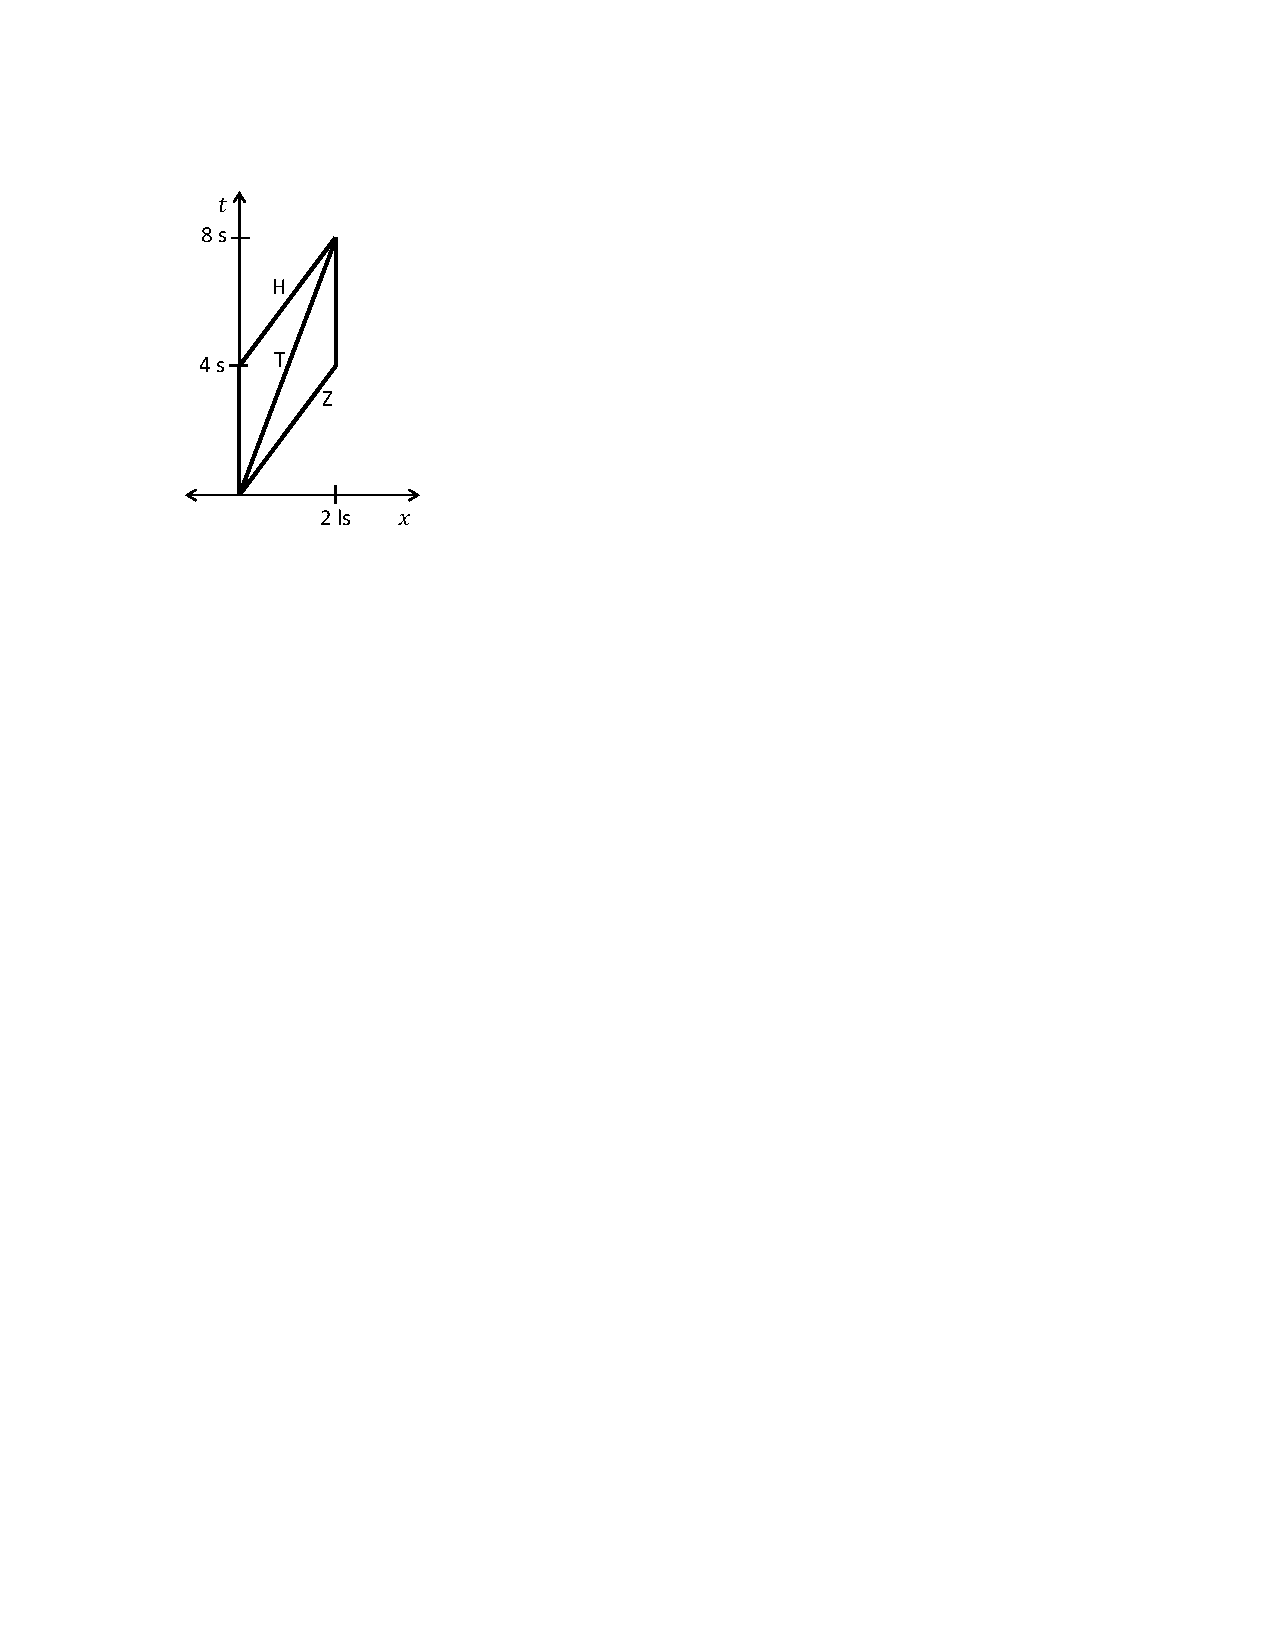
\includegraphics[scale=0.85]{M_problems/velocities_causality/tortoise_hare.pdf}

\end{minipage}

\begin{enumerate}[nosep,label=(\alph*)]
\item Draw a qualitative Minkowski diagram of the race in the reference frame of the tortoise.
\item How much time passes on the tortoise's wrist watch while he is running the race?
\item In the tortoise's reference frame, at what time does the zebra stop running, and at what time does the hare start running?  
\item According to the hare's wrist watch, how long does it take the hare to complete the course?  (The total time, including the time he was just standing around showboating.)
\item In the reference frame of the tortoise, what is the speed of the hare, once he starts running?
\end{enumerate}
At the end of the race, the zebra declares the race to be a tie.  The tortoise and hare each stare at their watches in amazement.  The other animals all boo and throw trash onto the field.  
\begin{enumerate}[resume*]
\item Do the tortoise, the hare, and the spectators agree or disagree about who crossed the finish line first?  Explain.
\item What do the tortoise, the hare, and the spectators measure for the time it took each competitor to complete the course?  (That's six times to compare.)  Do they agree or disagree about which competitor had the shortest time?  Again, explain.
\end{enumerate}
\end{Exercise}
\begin{Answer}
(b) 7.75 s (c) 3.61 s; 4.13 s (d) 7.48 s (e) $0.286c$ (f) They agree.  (g) As a check for your results, the sum of all six times is 46.46 seconds.  In fact, though their numbers differ, the tortoise, the hare, and all the other animals all agree on the ultimate outcome of the race, by any reasonable measure.  (The other animals only booed and threw trash on the field because they got caught up in the moment and it seemed like the right thing to do.)
\end{Answer}

\begin{Exercise}[difficulty=0]
Suppose you drive for 2 hours at 70 mph up to Washington DC, and then return back to Richmond at the same speed.  Due to time dilation, what is the difference between how much you aged, and how much your friend aged who stayed in Richmond? In answering this question, please do the calculation using a binomial series expansion for gamma, as in Lab~\ref{binomial_expansion_lab}.

\end{Exercise}
\begin{Answer}
The difference is 78 picoseconds.
\end{Answer}


\bigskip\bigskip
\pagebreak[3]
\textbf{Answers to Selected {\thesubsection} Problems:}
\label{lorentz_prob_answers}
%\shipoutExercise
\shipoutAnswer

\cleardoublepage

\subsection{Velocity, the Speed of Light, and Causality} 

(Answers to M\Alph{subsection} problems are on page \pageref{velocities_causality_prob_answers}.)


\begin{Exercise}[difficulty=0]
In class, we derived the ``forward'' velocity transformation, in which we find the velocity $u'$ of an object in a new frame $S'$,
$$
%u'=\frac{u-v}{1-\dfrac{uv}{c^2}}.
u'=\frac{u-v}{1-({uv}/{c^2})}.
$$
In this problem, you will derive the ``reverse'' velocity transformation, in which the velocity $u$ of an object in the frame $S$ is expressed in terms of $u'$ and $v$.  You will do this in three different ways. (a)~Use algebraic manipulation to solve the equation above for u. (b)~Start with the ``reverse'' Lorentz transformations $x=\gamma(x'+vt')$ and $t=\gamma[t'+(v/c^2 )x']$, and follow similar logic to what we did in class.  (c)~Use the trick you described in Problem \ref{fourth_lorentz_derivation_prob}.
\end{Exercise}


\begin{Exercise}[difficulty=1]
Event A occurs at coordinates $(x,ct)=(4~{\rm m},6~{\rm m})$.  Event B occurs at coordinates $(7$~m$,11$~m). (a)~What is the numerical value of the spacetime interval $(\Delta s)^2$ between your two points?  (b)~Is the spacetime interval between these events \textit{timelike}, \textit{spacelike}, or \textit{lightlike}, and how do you know?  
\end{Exercise}
\begin{Answer}
(a) $-16$~m$^2$  (b) timelike.  (Why?) 
\end{Answer}


\begin{Exercise}[difficulty=1]
Event A occurs at coordinates $(x,ct)=(2 {\rm m},-3 {\rm m})$.  (a)~Find any point B such that the spacetime interval between points A and B is lightlike.  (b)~What is the numerical value of the spacetime interval $(\Delta s)^2$ between your two points?
\end{Exercise}
\begin{Answer}
(b) 0
\end{Answer}


\begin{Exercise}[difficulty=0]
Anna, Bob, and their roommate Carlos are quarantined together in a small apartment, and they are starting to get on each other's nerves.  The space-time (Minkowski) diagram on the right shows three events that happen one afternoon, in the reference frame of their feckless cat, who is sleeping on the sofa.  The dotted lines on the graph represent the speed of light, as usual.

\begin{minipage}{0.55 \textwidth}
\begin{itemize}[nosep]
\item At point A, Anna hiccups.  
\item At point B, Bob emits a sudden snorting noise. 
\item At point C, Carlos spills his drink on his lap.  
\item Carlos says, ``Darn it, Bob, you made me spill my drink!''
\item Bob says, ``Sorry Carlos, but I only snorted because Anna startled me when she hiccupped.''
\end{itemize}

\bigskip

\begin{enumerate}[nosep,label=(\alph*),series=mylist]
\item Could Bob snorting have caused Carlos to spill his drink?  Explain.
\item Could Anna hiccupping have caused Bob to snort? Explain.
\end{enumerate}
\end{minipage}
\begin{minipage}{0.44 \textwidth}
\hspace{\fill}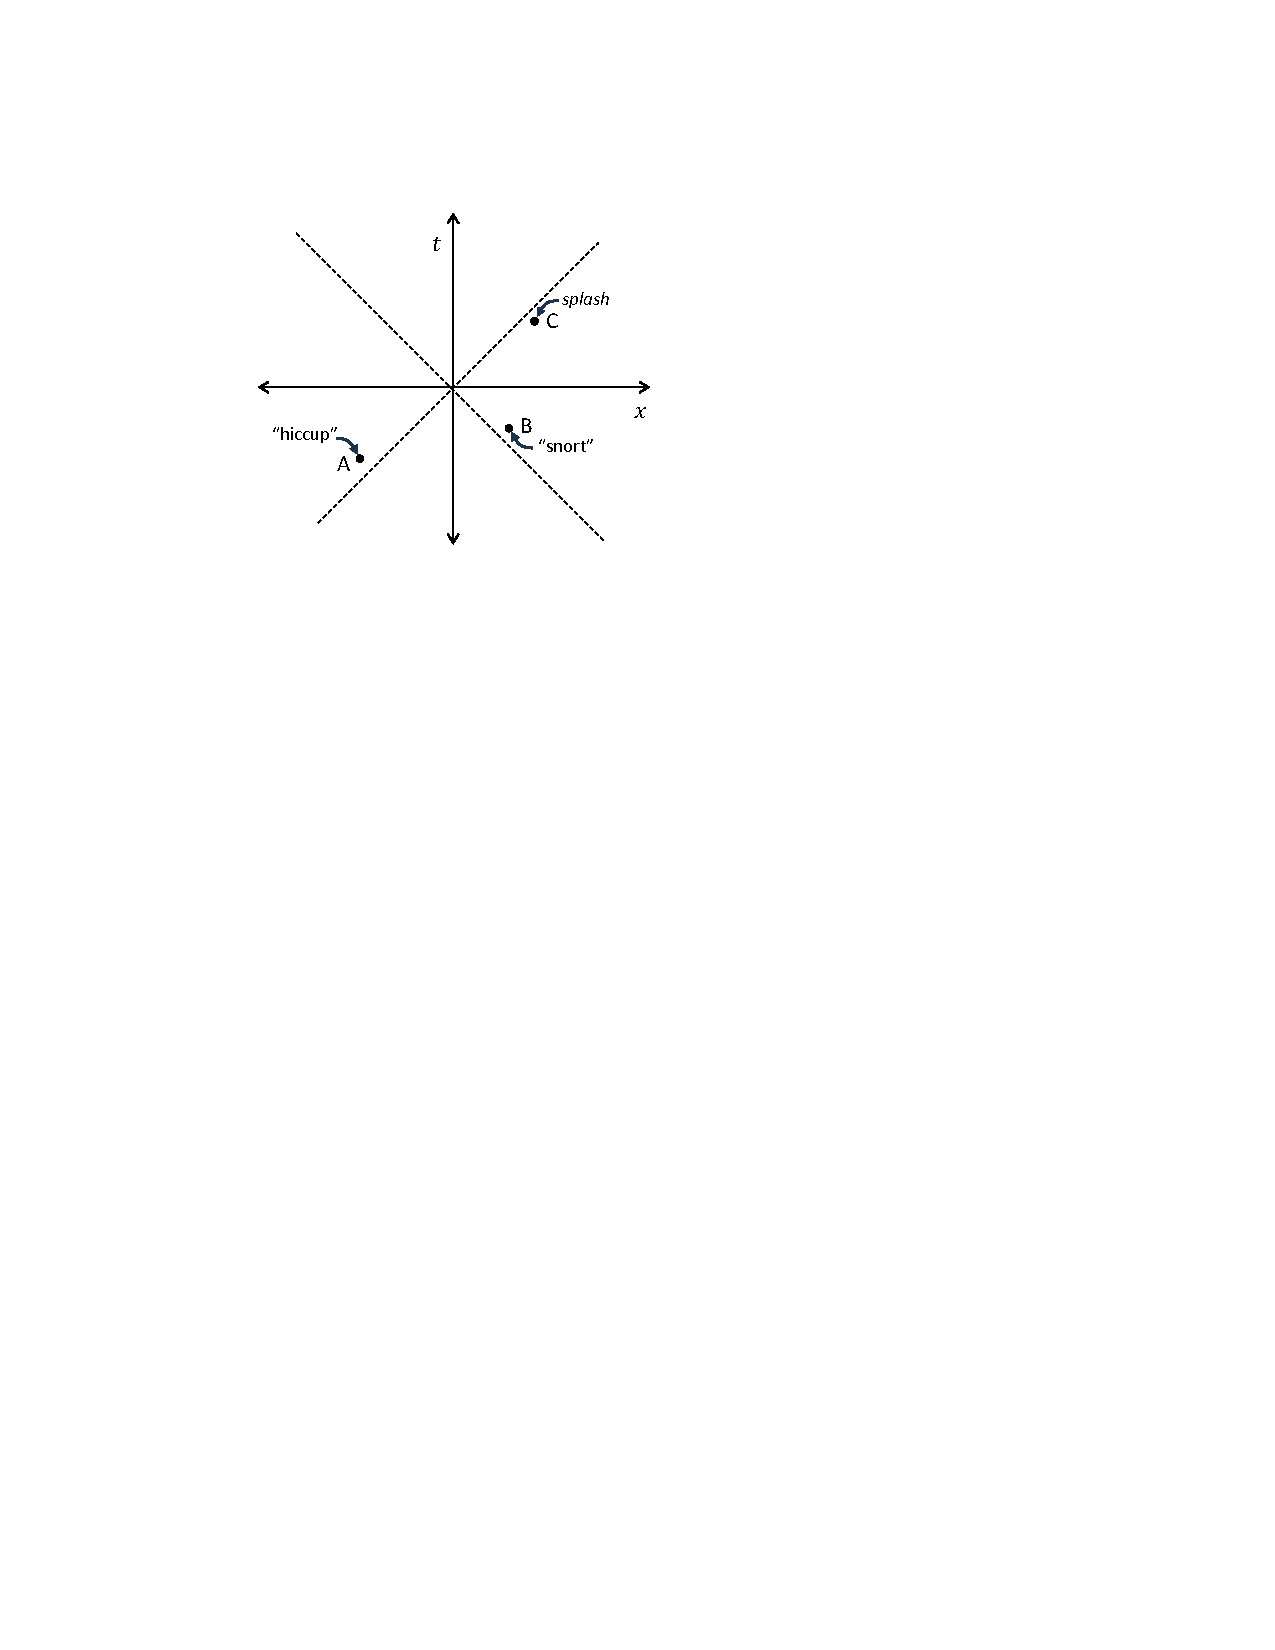
\includegraphics{M_problems/velocities_causality/hiccup_snort_splash.pdf}

\end{minipage}
\textit{Anna says, ``You are so full of it, Bob!  In case you didn't notice, I was traveling in the positive x-direction at a high velocity, and in my reference frame, you snorted before I hiccupped.  In fact, your snorting made me hiccup, so it's all your fault!''}
\begin{enumerate}[resume*=mylist] 
%There's a bug in enumitem that causes "resume" to fail when used in conjunction with minipage.  The fix is to use a named list (here "mylist").
\item Is it possible that Bob's snort happened before Anna's hiccup in Anna's reference frame? Explain.
\item Is it possible that Bob's snort caused Anna to hiccup?  Explain.
\end{enumerate}
\end{Exercise}
\begin{Answer}
(a) yes (b) no (c) yes (d) no
\end{Answer}


\begin{comment}
\begin{Exercise}[difficulty=1]
Two events occur at (x,ct) coordinates (4 m, 1 m) and (7 m, 6 m).  (a) Is the spacetime interval between these events timelike, spacelike, or lightlike?  (b) What is the proper time between these events?  (c) What is the proper distance between these two events?
\end{Exercise}
\begin{Answer}
MD6. (b) 4 m/c  (c) n/a
\end{Answer}



\begin{Exercise}[difficulty=1]
Two events occur at (x,ct) coordinates (-3 m, -2 m) and (7 m, 4 m).  (a) Is the spacetime interval between these events timelike, spacelike, or lightlike?  (b) What is the proper time between these events?  (c) What is the proper distance between these two events?
\end{Exercise}
\begin{Answer}
(a) spacelike (b) n/a (c) 8 m
\end{Answer}
\end{comment}




\bigskip\bigskip\bigskip
\pagebreak[3]
\textbf{Answers to Selected {\thesubsection} Problems:}
\label{velocities_causality_prob_answers}
%\shipoutExercise
\shipoutAnswer

\cleardoublepage
\subsection{Gravity and General Relativity} 

(Answers to M\Alph{subsection} problems are on page \pageref{gravity_prob_answers}.)


\begin{Exercise}[difficulty=0]
Suppose that you are closed inside a rocket with no windows, and no instruments except for a simple bathroom scale to stand on.  Now consider two scenarios drawn below: In scenario A, the rocket is at rest on the surface of the Earth, where the gravitational constant is $g=9.8~{\rm m/s}^2$. In scenario B, the rocket is far away from any stars or planets in interstellar space, and its engines are accelerating the rocket forwards at $a=g=9.8~{\rm m/s}^2$.
\begin{center}
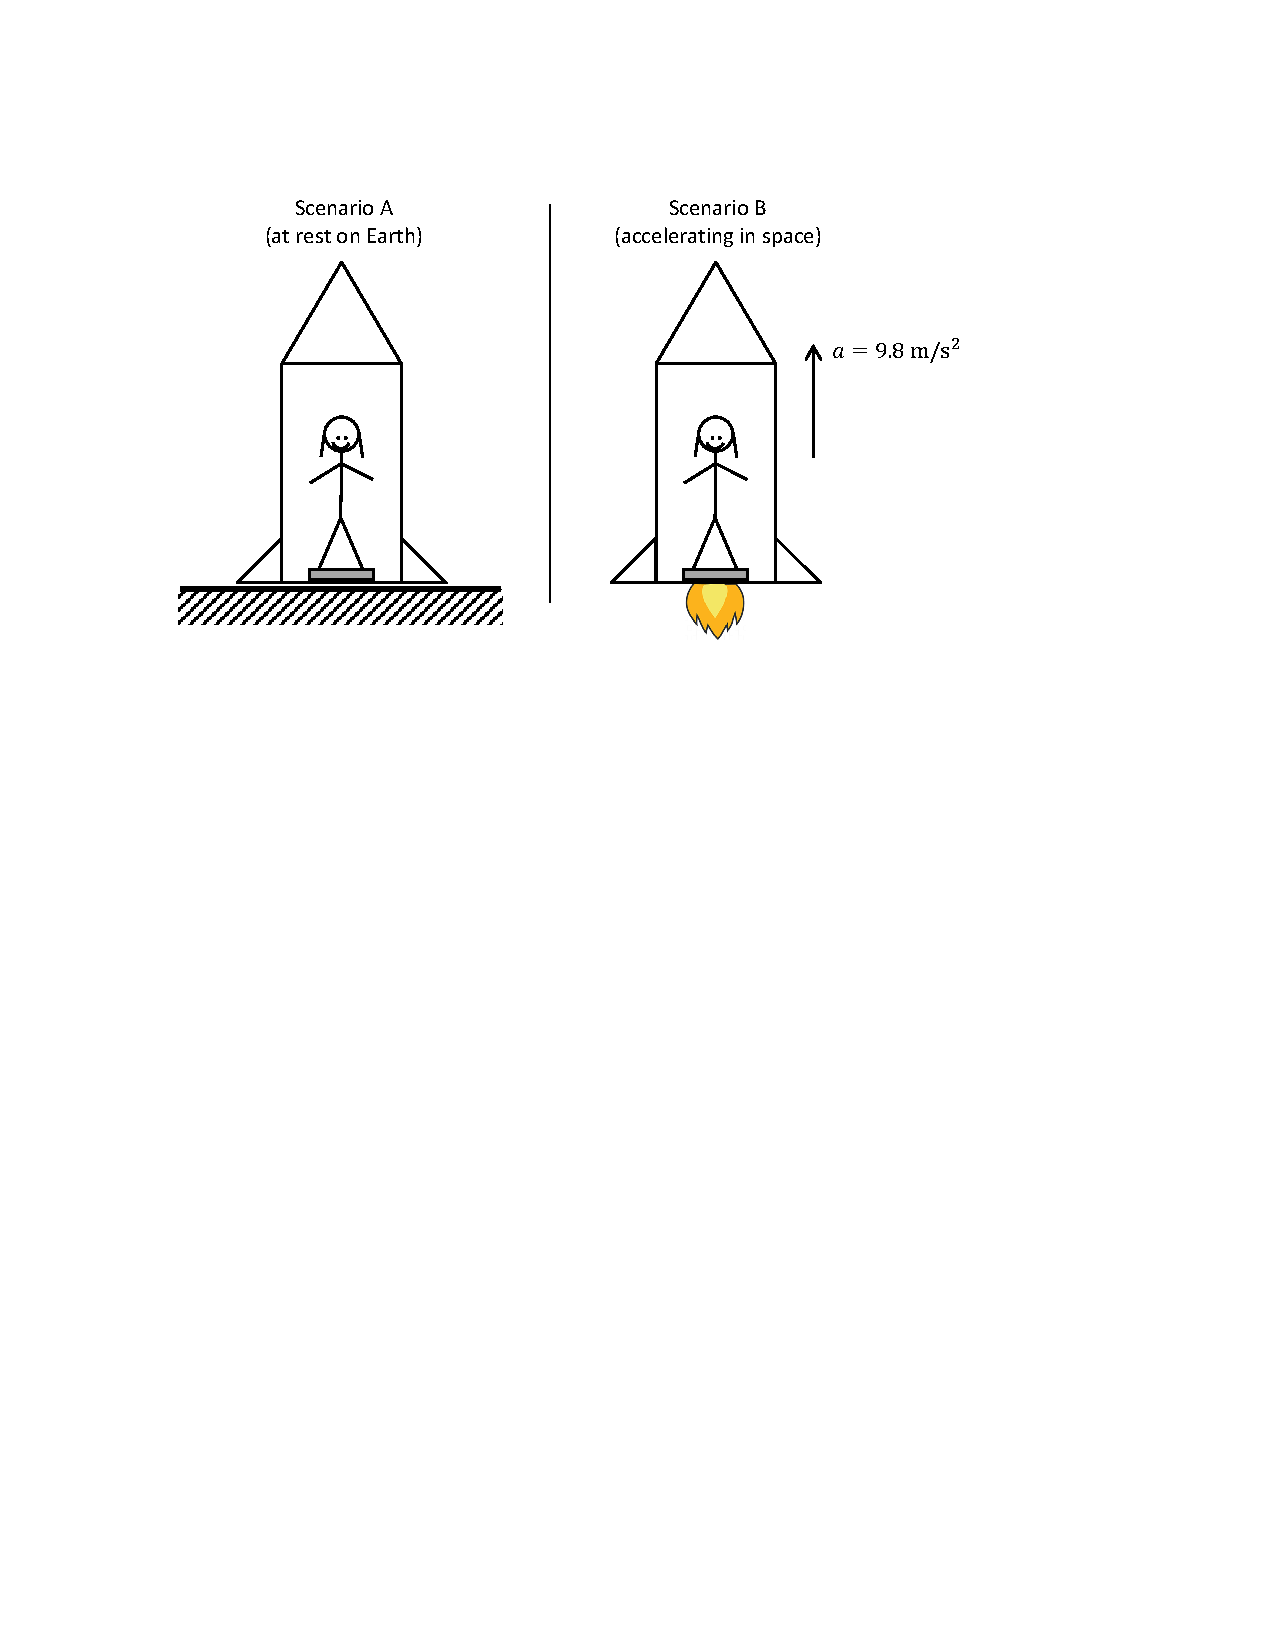
\includegraphics[scale=0.9]{M_problems/gravity/two_rockets_equivalence.pdf}
\index{color page}
\end{center}
(a) Draw a free-body diagram of \textit{you} in scenario A, and a free-body diagram of \textit{you} in scenario B.  In each case, draw vectors showing only the forces that are acting \textit{on you, directly,} not on the rocket ship.  (b)~If you were not told what situation you were in, could you tell the difference by standing on the bathroom scale and reading your ``weight''?  (c)~Suppose the engines were very, very quiet, so you could not hear or see whether they were on.  Would scenario A feel any different from scenario B?  If yes, how would it feel different?
\end{Exercise}


\begin{Exercise}[difficulty=0]
Congratulations!  You entered a raffle and have just won first prize: a one-week trip to Denver!\,\footnote{Second prize: two weeks.}  The elevation in Denver is roughly 1600 meters above sea level, hence its nickname, ``the mile-high city.''  If you spend a week in Denver, who ages more: you, or your friend who stays in Richmond? (Richmond is essentially at sea level.)  How large is this difference?
\end{Exercise}
\begin{Answer}
You age more than your friend in Richmond, and the difference you calculate should be close to 100 nanoseconds.
\end{Answer}

\begin{Exercise}[difficulty=0]
A very accurate atomic clock is placed on a jet plane, and an identical clock remains stationary on the ground.  The clock on the plane flies away from the stationary clock for five hours at the plane's standard cruise speed of 250~m/s at an altitude of 13000 m, then makes a U-turn and returns at the same speed and altitude.  What would be the difference in time measured between the two clocks at the end of the trip (a)~considering only time dilation related to the speed of the aircraft (special relativity), (b)~considering only time dilation due to gravity (general relativity), and (c)~considering both special and general relativity?  (d)~Which is the greater effect?
\end{Exercise}
\begin{Answer}
(a) 12.5 ns (b) 51 ns (c) 38.5 ns
\end{Answer}


\begin{Exercise}[difficulty=0]
\label{how_far_does_rocket_travel_prob}
In the example we did in class, we imagined a rocket with a light source at the bottom, and you as an observer at the top.  Suppose the rocket had a height of $H=20$~meters.  (a)~How long would it take light to travel the length of the rocket?  (b)~At an acceleration of $a=9.8~{\rm m/s}^2$, what would be the final speed of the rocket once the light reaches the top of the rocket, assuming the rocket starts at rest ($v=0$)?  (c)~What is the rocket's average speed during this time?  (Just $(v_{\rm initial} +v_{\rm final})/2$, that's all.)  (d)~At that average speed, how far does the rocket travel during this time?  (e)~In Activity 2 of Lab~\ref{gravity_time_lab}, we assumed that we could still treat the distance traveled by the light in our example as being approximately equal to the height of the rocket $H$.  Is that a reasonable approximation? 
\end{Exercise}
\begin{Answer}
(a) 66 ns (b) $6.5 \times 10^{-7}$~m/s (c) $3.27 \times 10^{-7}$ m/s (d) About 22 femtometers
\end{Answer}


\begin{minipage}{0.75 \textwidth}
\begin{Exercise}[difficulty=0]
A laser beam inside of a rocket ship is aimed exactly horizontally from one side of the ship to the other, hitting the opposite wall 4~meters away.  (a)~Suppose the ship is floating in space ($v=0$ in some reference frame), far away from any gravitational source.  At the moment the laser beam is turned on, the ship's engines fire, accelerating the ship forward at $a=9.8~{\rm m/s}^2$.  By what distance has the ship moved forward in the time it takes for the laser beam to cross the 4-meter width of the ship? (Hint: your work in Problem \ref{how_far_does_rocket_travel_prob} will be helpful here.)  (b)~Now suppose instead that the ship is standing motionless on the surface of the Earth.  By what vertical distance is the laser beam deflected down by the Earth's gravitational field?
\vspace{0.5in}
\end{Exercise}
\end{minipage}
\begin{minipage}{0.24 \textwidth}
\medskip
\hspace{\fill}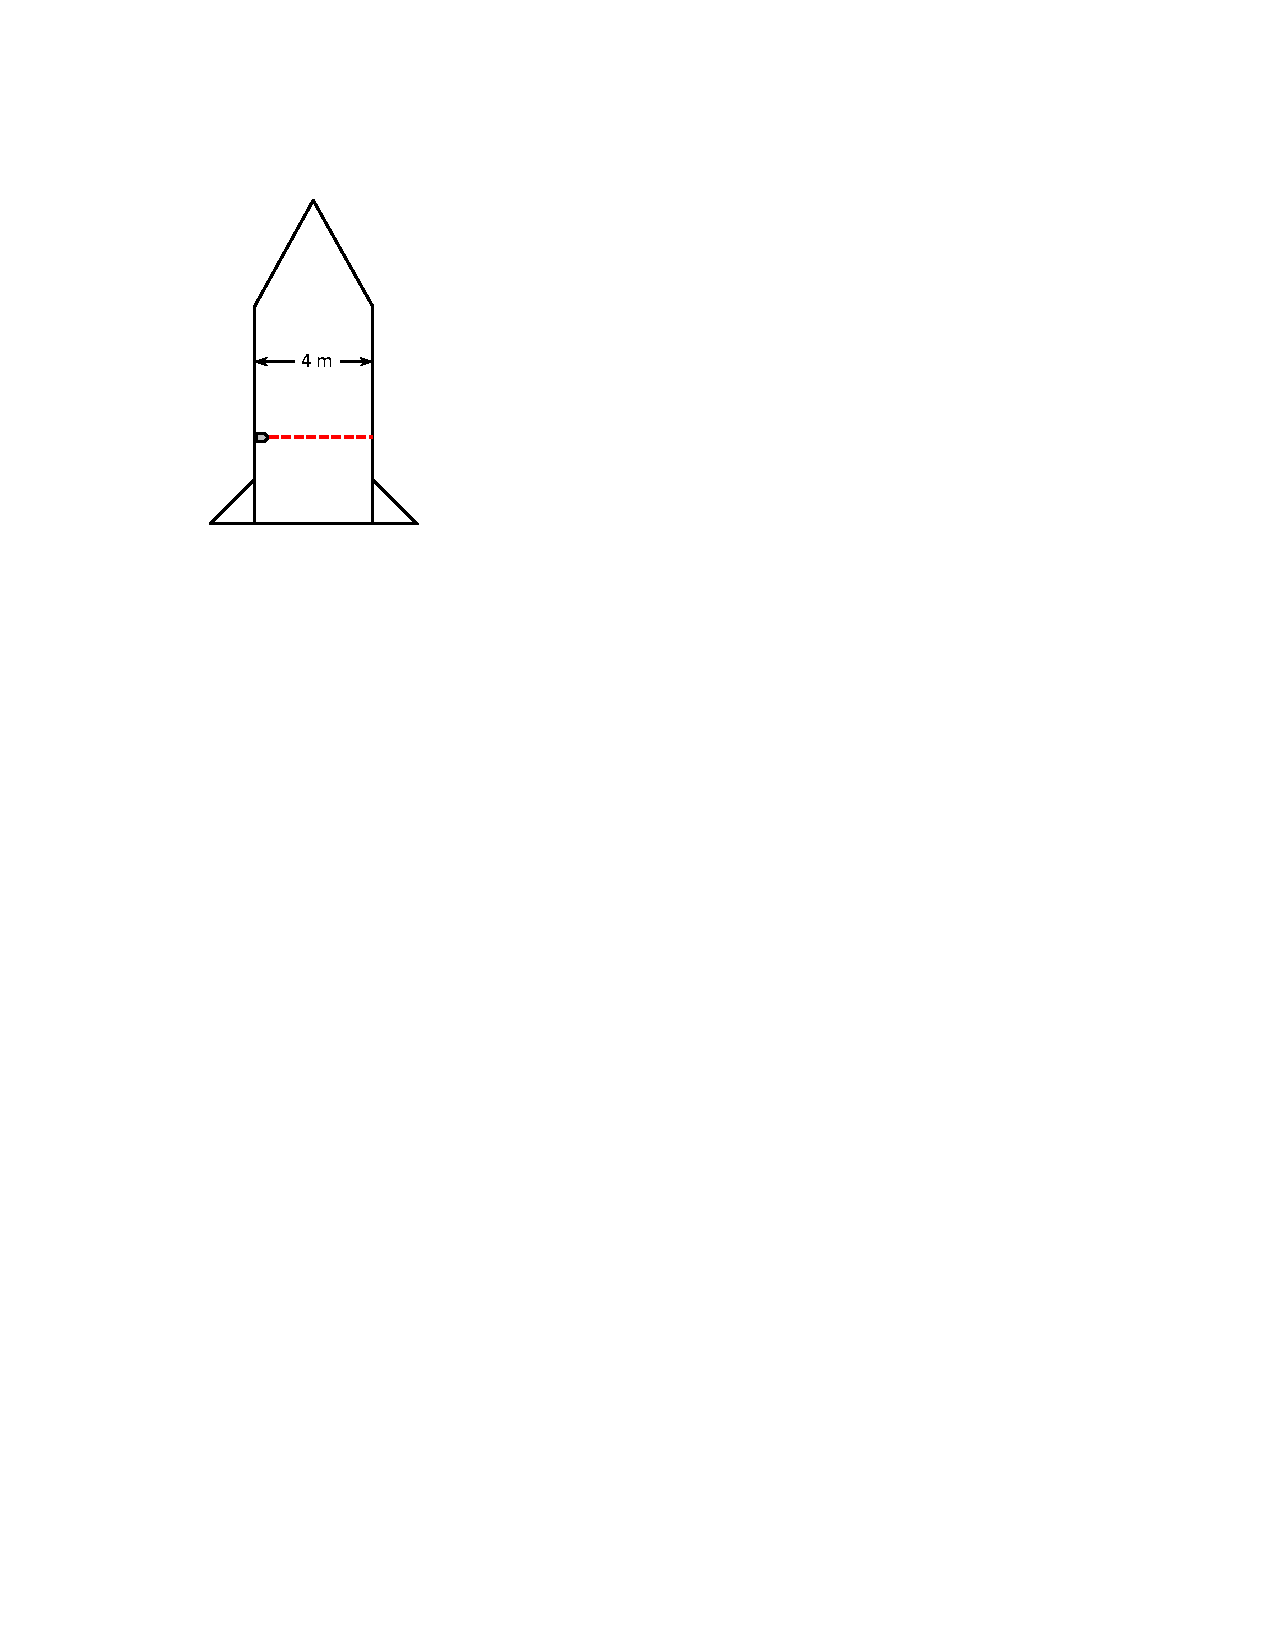
\includegraphics[scale=0.9]{M_problems/gravity/rocket_and_horizontal_laser.pdf}
\index{color page}
\end{minipage}
\begin{Answer}
(b) 0.88 femtometers
\end{Answer}





\bigskip\bigskip\bigskip
\pagebreak[3]
\textbf{Answers to Selected {\thesubsection} Problems:}
\label{gravity_prob_answers}
%\shipoutExercise
\shipoutAnswer

\cleardoublepage
\subsection{Energy and Mass} 

(Answers to M\Alph{subsection} problems are on page \pageref{energy_mass_prob_answers}.)


\begin{Exercise}[difficulty=1]
\label{problem_ball_and_cliff_basic}
Anna and Bob, curious about conservation of energy, head to a 10-meter-high cliff, armed with a 4~kg bowling ball.  Bob drops the bowling ball from the top of the cliff; as it falls, 392 joules of gravitational potential energy are converted to kinetic energy $K$ of the bowling ball.  What is the final speed of the ball at the bottom of the cliff, just before it hits the ground?
\end{Exercise}
\begin{Answer}
14 m/s
\end{Answer}

\begin{Exercise}[difficulty=1]
\label{problem_ball_and_cliff_trampoline}
Anna and Bob decide to drop the bowling ball off the cliff again, as they did in 
Problem~\ref{problem_ball_and_cliff_basic}.  This time, Anna places a large trampoline at the bottom of the 10-meter cliff, and Bob drops the bowling ball so that it lands directly on the trampoline.  The ball depresses the center of the trampoline and then bounces back up roughly to Bob's height.  Anna notices that when the bowling ball is at its lowest point, the springs on the edges of the trampoline are all visibly stretched.  How much potential energy is stored in the springs at the moment when they are at their maximum stretch?
\end{Exercise}
\begin{Answer}
392 J
\end{Answer}


\begin{Exercise}[difficulty=0]
Anna and Bob do one final experiment at the same cliff in Problems~\ref{problem_ball_and_cliff_basic} and \ref{problem_ball_and_cliff_trampoline}.  At the top of the cliff, instead of simply dropping the ball, Bob throws the ball directly downward, giving it an initial speed of $v_i=6$~m/s.  (a)~How much kinetic energy did Bob add to the bowling ball with his throwing motion?  (b)~What is the final velocity of the ball at the bottom of the cliff, just before it hits the ground (or the trampoline)?
\end{Exercise}
\begin{Answer}
(a) 72 J (b) 15.2 m/s
\end{Answer}



\begin{Exercise}[difficulty=0]
\label{prob_K_at_low_and_high_speeds}
A helium atom has a mass of $m=6.68 \times 10^{-27}$~kg.  Use both the Newtonian expression $K=\frac{1}{2} mv^2$ and the relativistic expression $K=(\gamma -1)mc^2$ to calculate the kinetic energy of the helium atom (a)~at $v=0.008c$ (b)~at $v=0.08c$, and (c)~at $v=0.8c$.
\end{Exercise}
\begin{Answer}
(a)~$1.9238 \times 10^{-14}$~J, $1.9239 \times 10^{-14}$~J  
(b)~$1.9238 \times 10^{-12}$~J, $1.9331 \times 10^{-12}$~J  
(c)~$1.9238 \times 10^{-10}$~J, $4.008 \times 10^{-10}$~J
\end{Answer}


\begin{Exercise}[difficulty=0]
You've just seen in Problem~\ref{prob_K_at_low_and_high_speeds} that for low speeds ($v \ll c$), the Newtonian expression and the relativistic expression for kinetic energy yield similar results.  Now, you'll prove it.  (a)~Write the relativistic expression for kinetic energy $K$, but do so by writing out $\gamma$ in terms of $v$ and $c$.  (That is, just substitute in the equation for $\gamma$.)  (b)~Rewrite the relativistic expression for $K$ using an exponent of $-\frac{1}{2}$ rather than a square root sign, and use the binomial series expansion $(1+x)^\alpha \approx 1+\alpha x$ to expand $\gamma$.  (See Lab~\ref{binomial_expansion_lab}.  We'll assume here that $v/c \ll 1$, so that you only need to keep the first two terms of the expansion, ignoring anything of order $x^2$ or higher.)  (c)~Show that your result reduces to the Newtonian result~$K=\frac{1}{2} mv^2$.
\end{Exercise}


\begin{minipage}{0.60 \textwidth}
\begin{Exercise}[difficulty=0]
\label{prob_collision_2m_and_m}
Two particles of different masses collide together.  The first particle has a mass $2m$ and speed $u_1=0.5c$.  The second particle has a mass of $m$ (half the first mass) and a speed of $u_2=0.756c$ in the opposite direction.  When they collide and stick together, the resulting particle is at rest, with velocity $u_{\rm f}=0$.  (a)~What is the mass $M$ of the resulting particle?  (b)~How much kinetic energy is converted to mass during the collision?
\end{Exercise}
\end{minipage}
\begin{minipage}{0.39 \textwidth}
\hspace{\fill}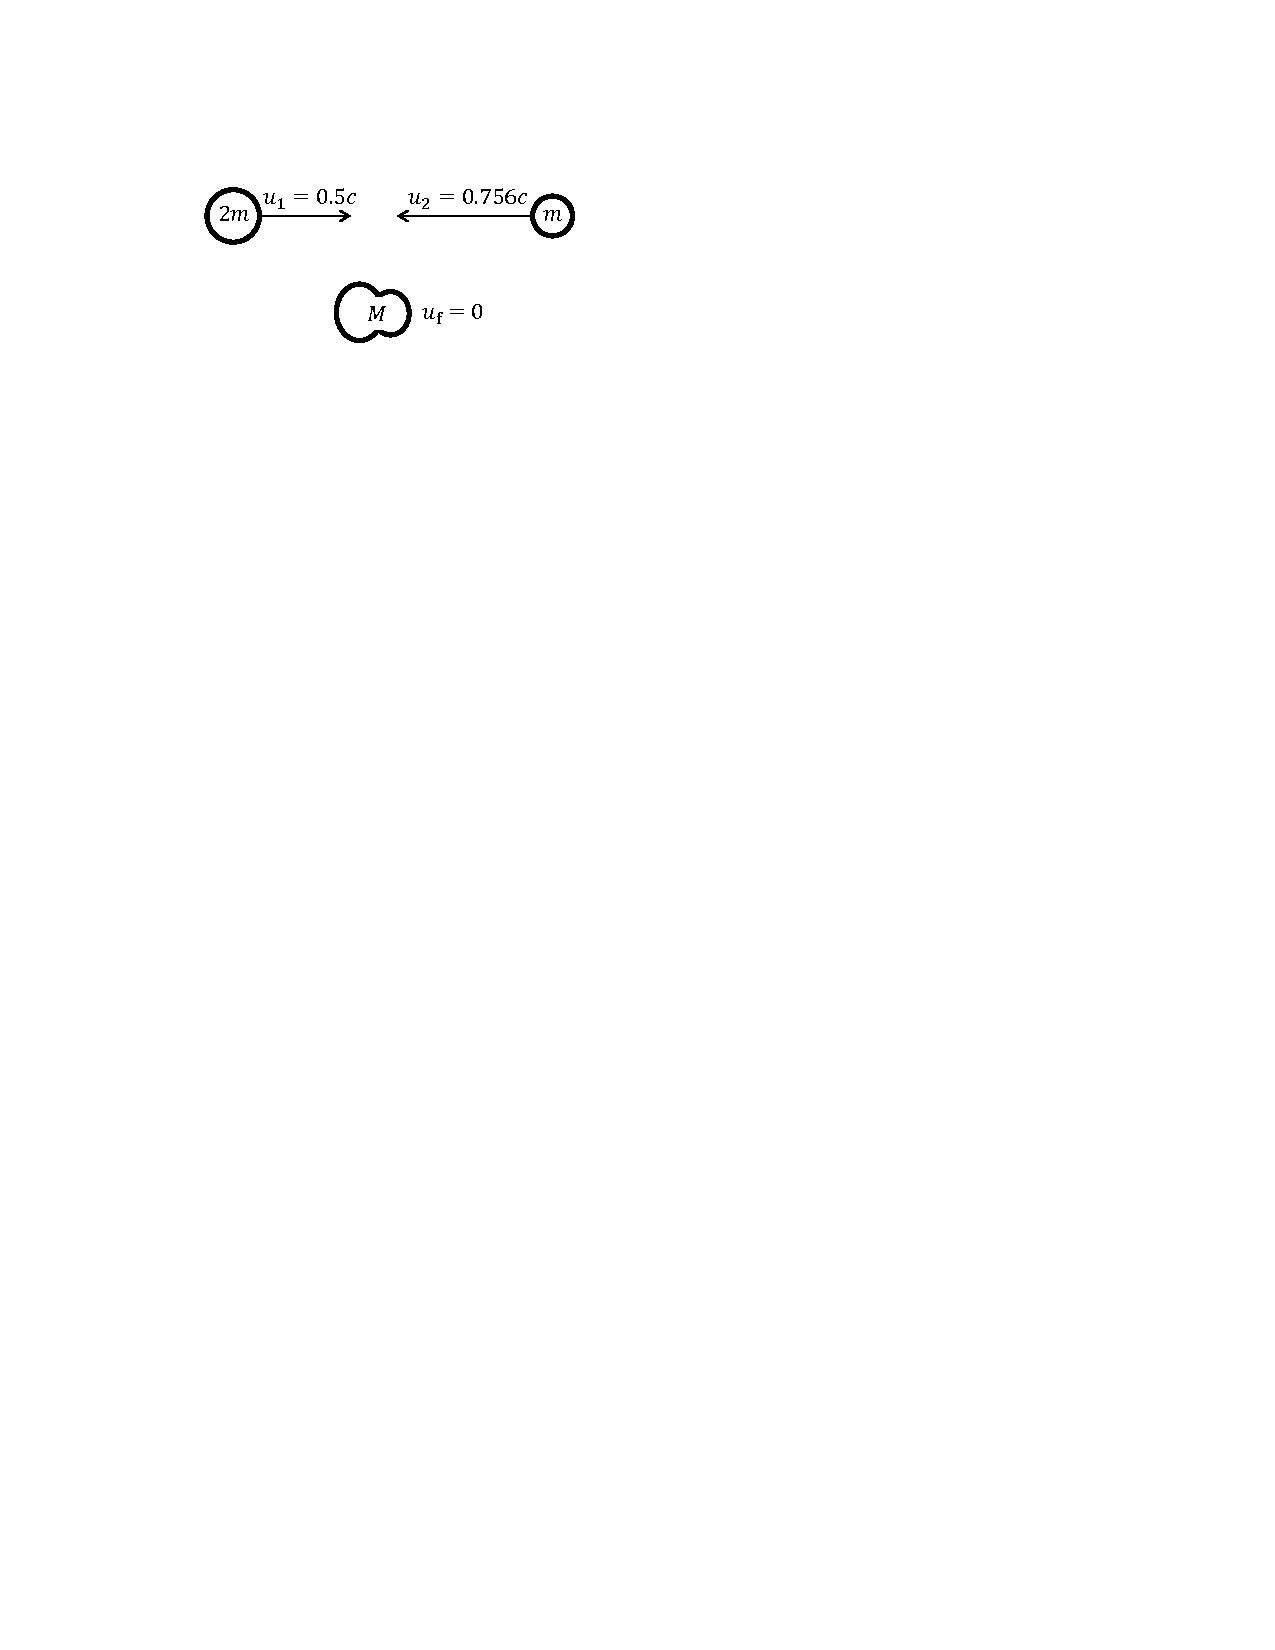
\includegraphics[scale=0.9]{M_problems/energy_mass/collision_m_and_2m.pdf}
\end{minipage}
\begin{Answer}
(a) $3.84m$ (b) $0.84mc^2$
\end{Answer}


\begin{Exercise}[difficulty=0]
In this problem, we'll analyze the collision of Problem~\ref{prob_collision_2m_and_m} in a reference frame with speed $v=0.5c$, in which the first particle now has speed $u_1=0$.  (a)~What are the speeds of the other original particle and the resulting particle in this reference frame?  (b)~What is the initial kinetic energy of the system before the collision?  (c)~What is the final kinetic energy of the system after the collision?  (d) What is the total energy $E_{\rm total}$ of the system in this reference frame?
\end{Exercise}
\begin{Answer}
(a) $0.911c$, $0.5c$ (b) $1.43mc^2$ (c) $0.59mc^2$ (d) $4.43mc^2$
\end{Answer}


\begin{Exercise}[difficulty=0]
In Problem \ref{problem_ball_and_cliff_trampoline}, Bob dropped a 4~kg bowling ball from a height of 10~meters onto a trampoline, visibly stretching its springs.  By how much did the mass of the springs change, and did they become heavier or lighter?
\end{Exercise}
\begin{Answer}
The springs' mass increases by $4.35 \times 10^{-15}$~kg.
\end{Answer}


\begin{minipage}{0.60 \textwidth}
\begin{Exercise}[difficulty=0]
In one of the common reactions late in a star's life cycle, nitrogen and hydrogen combine to produce one carbon atom and one helium atom:
$$
\isotope[15][7]{N} + \isotope[1][1]{H} \longrightarrow \isotope[12][6]{C} + \isotope[4][2]{He}.
$$
How much energy is given off by this reaction?  The table to the right lists the masses of each isotope in atomic mass units (amu), where $1~{\rm amu}=931.494~{\rm MeV}/c^2$.  (See Appendix~\ref{appendix_nuclear_primer} for an explanation of the isotope notation in the table.)
\end{Exercise}
\end{minipage}
\begin{minipage}{0.39 \textwidth}
\hspace{\fill}
{\renewcommand{\arraystretch}{1.5}
\begin{tabular}{|C{0.8in}|C{1.0in}|} \hline 
\textbf{Isotope} & \textbf{Mass (in amu)} \\ 
\hhline{|=|=|}
 \isotope[1][1]{H} & 1.007825 \\ \hline 
 \isotope[4][2]{He} & 4.002603 \\ \hline 
 \isotope[12][6]{C} & 12.0000000 \\ \hline 
 \isotope[15][7]{N} & 15.0001089 \\ \hline 
\end{tabular} }

\end{minipage}
\begin{Answer}
4.96 MeV
\end{Answer}


\begin{Exercise}[difficulty=0]
A typical large nuclear reactor produces about 1000 megawatts of electrical power, enough to power between 500,000 and 1,000,000 homes.  Over the course of a year, a reactor like that produces about $3 \times 10^{16}$~joules of energy.  Keeping it running requires about 30 metric tons (30,000~kg) of uranium, formed into pellets and stacked into fuel rods.  The rods are replaced every few years.  How much does the total mass of these rods change over the course of one year?  Do the rods become lighter or heavier?
\end{Exercise}
\begin{Answer}
The rods become lighter, by about a third of a kilogram.  Incidentally, a similarly-sized coal-burning plant burns more like 2,000,000 metric tons ($2 \times 10^9$~kg) of coal per year, most of which ends up as carbon dioxide in our atmosphere.
\end{Answer}




\bigskip\bigskip\bigskip
\pagebreak[3]
\textbf{Answers to Selected {\thesubsection} Problems:}
\label{energy_mass_prob_answers}
%\shipoutExercise
\shipoutAnswer

\cleardoublepage
\subsection{More Examples} 

(Answers to M\Alph{subsection} problems are on page \pageref{examples_prob_answers}.)



\begin{Exercise}
The graph below shows the number of decays of the excited state \isotope[137\mathrm{m}][56]{Ba} measured as a function of time, just as you did in Lab~\ref{nuclear_decay_lab}. (a)~Estimate by eye the half-life $t_{1/2}$ of the excited state of \isotope[137{\rm m}]{Ba} from the graph below. (I don't want you actually calculate anything.  I want you to think about what ``half-life'' means and give me a rough value for it.)  (b)~Estimate by eye the ``mean lifetime'' $\tau$ from the graph below.  (c)~Based on your previous answer, estimate the value of the decay constant $\lambda$, including the correct units. (Bear in mind that this $\lambda$ has nothing to do with any wavelength, other than that they happen to use the same Greek letter.) 
\begin{center}
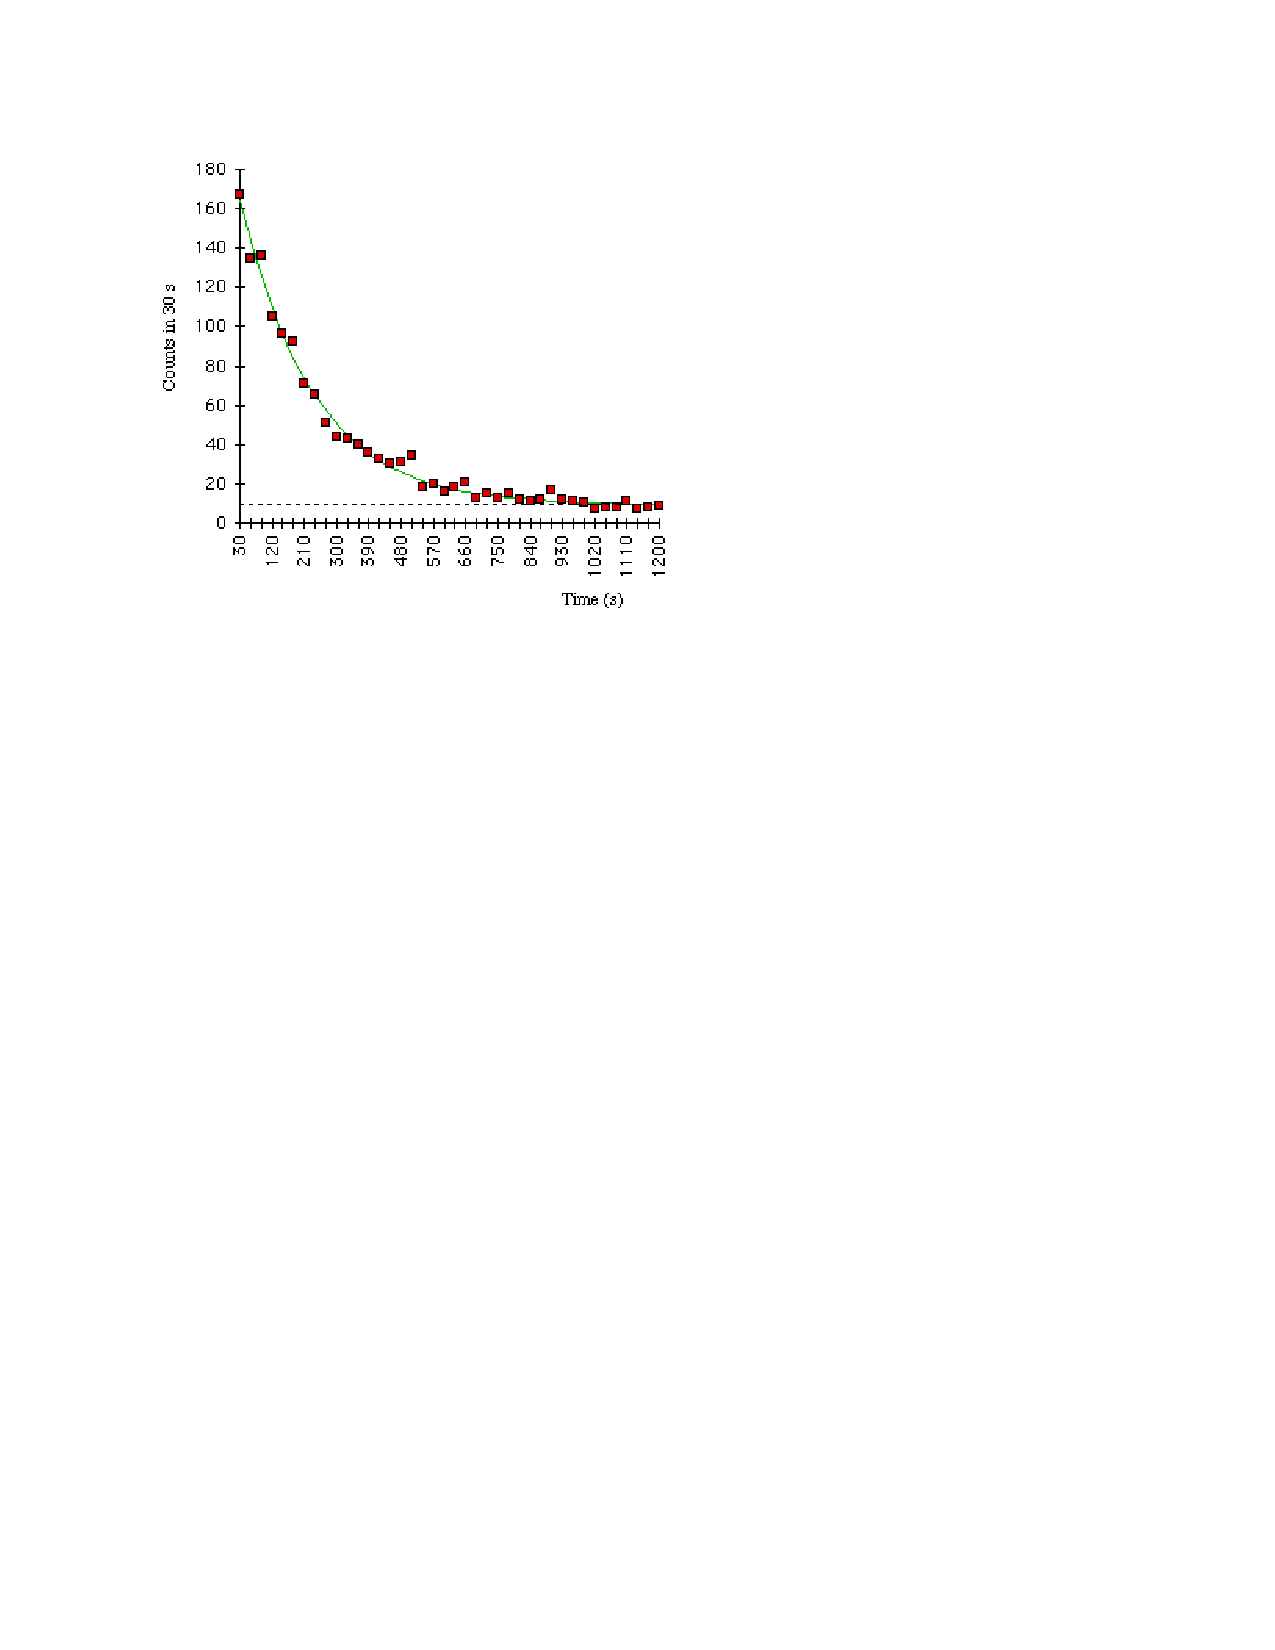
\includegraphics{M_problems/lorentz/barium_decay_graph.pdf}
\index{color page}
\end{center}
 \end{Exercise}
\begin{Answer}
(a) About 210 seconds (b) About 300 seconds (c) $\approx 3.3 \times 10^{-3}~{\rm s}^{-1}$
\end{Answer}

\begin{Exercise}
The radioactive isotope \isotope[15]{C} has a half-life of 2.449~seconds.  (a)~Calculate the mean lifetime $\tau$ and decay constant $\lambda$ for \isotope[15]{C}.  (b)~Suppose you begin at time $t=0$ with a sample of $N_0=10,000$ atoms of \isotope[15]{C}.  How many atoms $N$ do you expect to be left at time $t=8$ seconds?  (c)~What percent of the original atoms (that is, $N/N_0$, expressed as a percentage) would you expect to remain at time $t=11$~seconds?
\end{Exercise}
\begin{Answer}
(a) $\tau=3.53$~s, $\lambda=0.283~{\rm s}^{-1}$  (b)~About 1039 atoms, though due to statistical fluctuations it might be a little higher or lower, in the same way that if you flipped 10,000 coins, you might end up with results slightly different from 5000 heads and 5000 tails.  (c)~4.4\%
\end{Answer}


\begin{Exercise}
At rest, neutrons that are not bound within atomic nuclei have a mean lifetime of $\tau=14.692$~minutes.  The fusion of deuterium and tritium nuclei (\isotope[2]{H} and \isotope[3]{H}, respectively), in a laboratory or in the sun, produces helium (\isotope[4]{He}) and a very high-energy neutron that travels at 17.3\% of the speed of light.  What is the mean lifetime of these fast neutrons, in seconds, in the ``laboratory'' reference frame (that is, the reference frame of the Earth)?  You'll need to keep five significant digits in your answer, to make it clear that your answer is different from the 
14.692~minutes in the reference frame of the neutron.
\end{Exercise}
\begin{Answer}
894.99 seconds.
\end{Answer}

\begin{Exercise}[difficulty=0]
Anna has recently taken up pole vaulting, and owns a 10~m long pole (its proper length).  Bob has taken up farming, and owns an 8~m long barn (also its proper length) with a door on each end.  Anna runs very fast towards the open barn; in fact, she runs so fast that in the reference frame of Bob and the barn, the pole's length is Lorentz contracted to just 6~meters.  When Bob sees that Anna is exactly centered inside the barn, he pushes a button that closes both doors very quickly.  
\begin{itemize}
\item Bob says, ``Hah! I've closed Anna and her pole inside my barn!''  
\item But in Anna's reference frame, it is the barn that is Lorentz contracted.  Anna says, ``My pole is 10 meters long, and your dinky little barn is clearly less than 8 meters long.  Since your barn is shorter than my pole, you couldn't possibly close me and my pole inside of it!''
\end{itemize}
\begin{center}
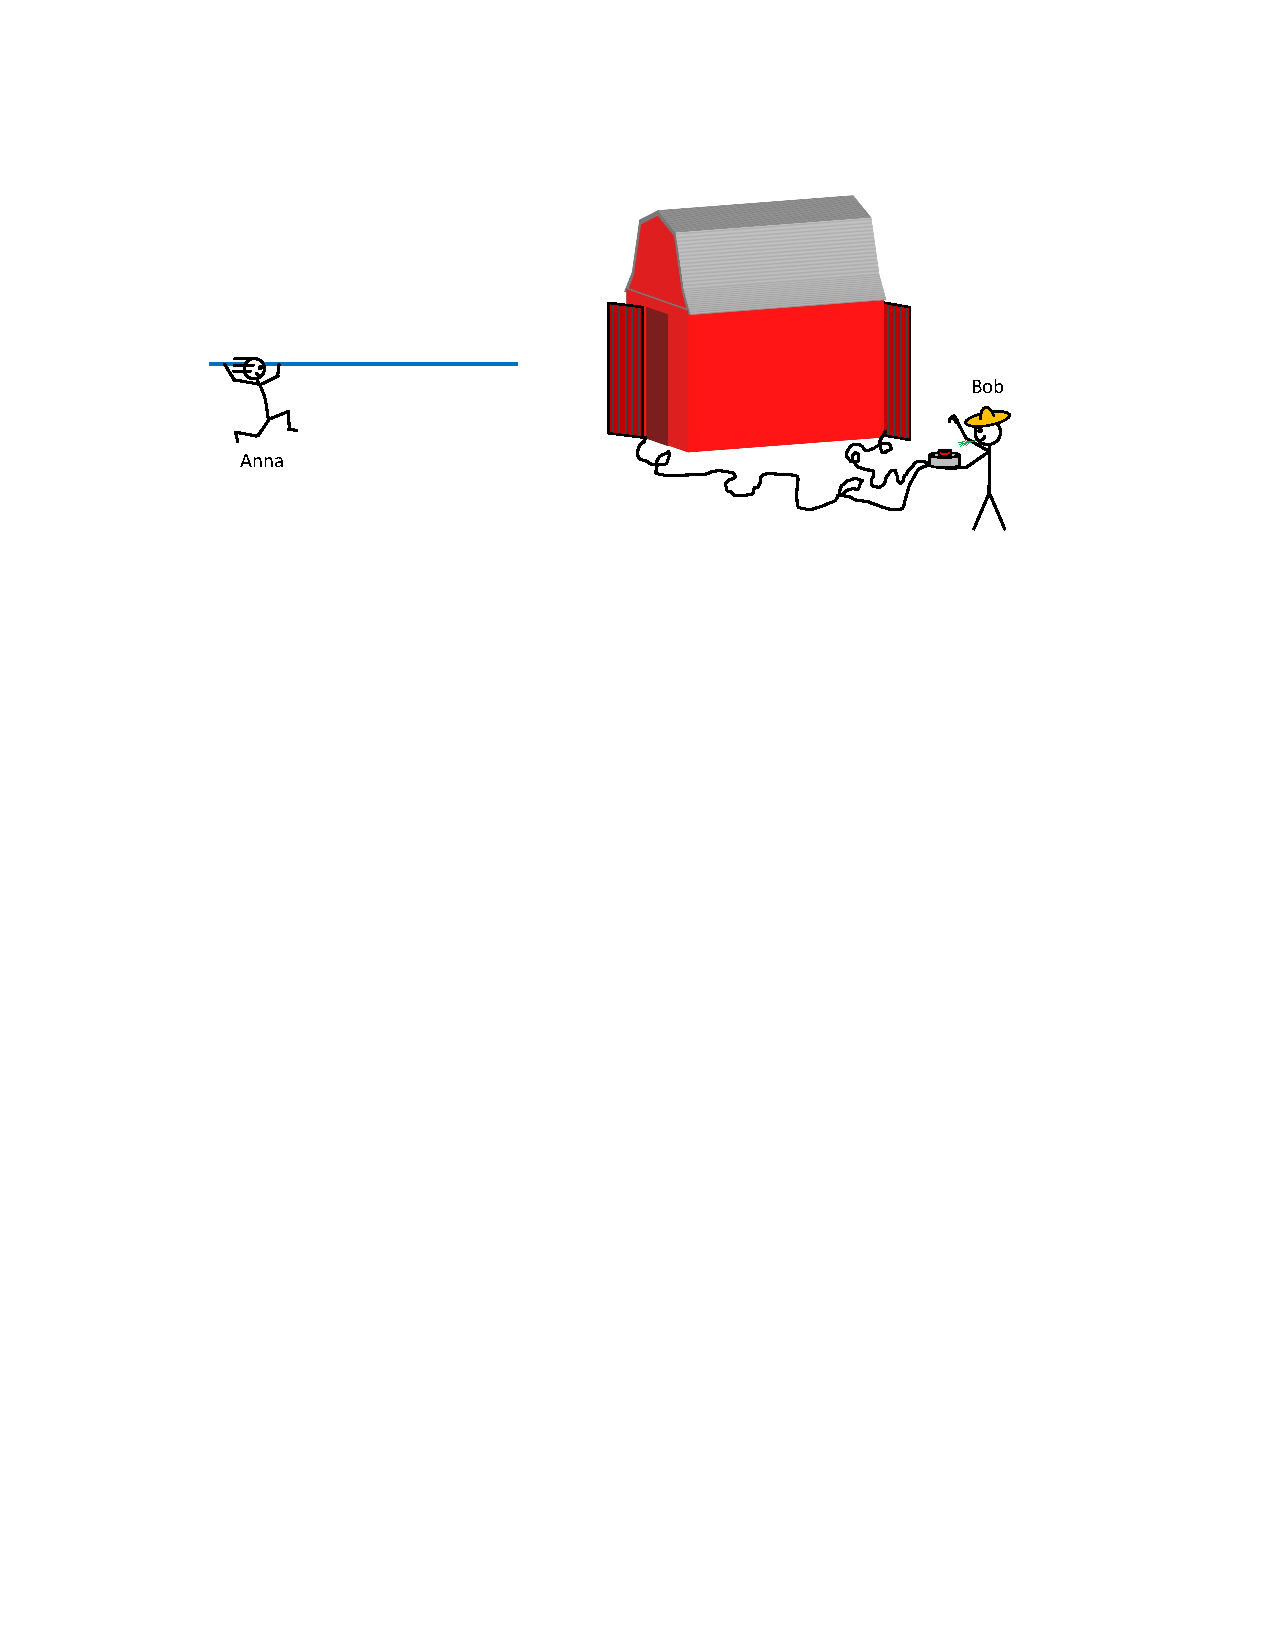
\includegraphics[scale=0.85]{M_problems/velocities_causality/pole_and_barn_color.pdf}
\index{color page}
\end{center}
Who is correct?  Anna, or Bob?  (Remarks: this problem is actually quite tricky, and we'll address it in our next class.  Take five or ten minutes to think about it and write down your thoughts, but don't spend more time on it than that.)
\end{Exercise}



\begin{Exercise}[difficulty=0]
Bob and Anna are the same age.  While Bob stays on Earth, Anna sets off at a constant speed $v=0.8c$ ($\gamma=1.67$) to visit another planet.  In the Earth reference frame, the planet is 24~ly away.  Once there, she turns around and comes back, also at $v=0.8c$.  (a) According to Bob, how long is Anna gone?  (b) According to Anna, how long is she gone?  (c) Suppose that instead of staying on Earth, Bob is floating in a spaceship (engines off) just outside our solar system during Anna's journey.  Does this affect your answers to parts (a) and (b)?  (d) Suppose that instead of traveling to a specific planet, Anna simply travels away in a random direction to a distance 24 ly away from Bob (according to Bob).  Does that change your answers to parts (a) and (b)?  (e) Just before they reunite, Anna radios Bob, saying ``Hey, from my spaceship, it looks like you had a velocity of $0.8c$ away from me, and then you turned around and had a velocity of $0.8c$ towards me.  I expect that when I see you again, you will not have aged as much, and will look much younger than me.''  Bob expects Anna to be younger.  But Anna also expects Bob to be younger.  Can they both be right?  Explain how to resolve this apparent paradox.
\end{Exercise}
\begin{Answer}
(a) 60 years (b) 36 years
\end{Answer}





\bigskip\bigskip\bigskip
\pagebreak[3]
\textbf{Answers to Selected {\thesubsection} Problems:}
\label{examples_prob_answers}
%\shipoutExercise
\shipoutAnswer

\cleardoublepage
